% Generated by Sphinx.
\def\sphinxdocclass{report}
\documentclass[a4paper,12pt,ngerman]{sphinxmanual}
\usepackage[utf8]{inputenc}
\DeclareUnicodeCharacter{00A0}{\nobreakspace}
\usepackage{cmap}
\usepackage[T1]{fontenc}
\usepackage{babel}
\usepackage{times}
\usepackage[Sonny]{fncychap}
\usepackage{longtable}
\usepackage{sphinx}
\usepackage{multirow}
\setcounter{tocdepth}{0}

\title{Übung zu Grundzüge der Geoinformation}
\date{03.03.2015}
\release{}
\author{Markus Mayr}
\newcommand{\sphinxlogo}{
\includegraphics{geoinfo_logo_sm.png}\par}
\renewcommand{\releasename}{Release}
\makeindex

\makeatletter
\def\PYG@reset{\let\PYG@it=\relax \let\PYG@bf=\relax%
    \let\PYG@ul=\relax \let\PYG@tc=\relax%
    \let\PYG@bc=\relax \let\PYG@ff=\relax}
\def\PYG@tok#1{\csname PYG@tok@#1\endcsname}
\def\PYG@toks#1+{\ifx\relax#1\empty\else%
    \PYG@tok{#1}\expandafter\PYG@toks\fi}
\def\PYG@do#1{\PYG@bc{\PYG@tc{\PYG@ul{%
    \PYG@it{\PYG@bf{\PYG@ff{#1}}}}}}}
\def\PYG#1#2{\PYG@reset\PYG@toks#1+\relax+\PYG@do{#2}}

\expandafter\def\csname PYG@tok@gd\endcsname{\def\PYG@tc##1{\textcolor[rgb]{0.63,0.00,0.00}{##1}}}
\expandafter\def\csname PYG@tok@gu\endcsname{\let\PYG@bf=\textbf\def\PYG@tc##1{\textcolor[rgb]{0.50,0.00,0.50}{##1}}}
\expandafter\def\csname PYG@tok@gt\endcsname{\def\PYG@tc##1{\textcolor[rgb]{0.00,0.27,0.87}{##1}}}
\expandafter\def\csname PYG@tok@gs\endcsname{\let\PYG@bf=\textbf}
\expandafter\def\csname PYG@tok@gr\endcsname{\def\PYG@tc##1{\textcolor[rgb]{1.00,0.00,0.00}{##1}}}
\expandafter\def\csname PYG@tok@cm\endcsname{\let\PYG@it=\textit\def\PYG@tc##1{\textcolor[rgb]{0.25,0.50,0.56}{##1}}}
\expandafter\def\csname PYG@tok@vg\endcsname{\def\PYG@tc##1{\textcolor[rgb]{0.73,0.38,0.84}{##1}}}
\expandafter\def\csname PYG@tok@m\endcsname{\def\PYG@tc##1{\textcolor[rgb]{0.13,0.50,0.31}{##1}}}
\expandafter\def\csname PYG@tok@mh\endcsname{\def\PYG@tc##1{\textcolor[rgb]{0.13,0.50,0.31}{##1}}}
\expandafter\def\csname PYG@tok@cs\endcsname{\def\PYG@tc##1{\textcolor[rgb]{0.25,0.50,0.56}{##1}}\def\PYG@bc##1{\setlength{\fboxsep}{0pt}\colorbox[rgb]{1.00,0.94,0.94}{\strut ##1}}}
\expandafter\def\csname PYG@tok@ge\endcsname{\let\PYG@it=\textit}
\expandafter\def\csname PYG@tok@vc\endcsname{\def\PYG@tc##1{\textcolor[rgb]{0.73,0.38,0.84}{##1}}}
\expandafter\def\csname PYG@tok@il\endcsname{\def\PYG@tc##1{\textcolor[rgb]{0.13,0.50,0.31}{##1}}}
\expandafter\def\csname PYG@tok@go\endcsname{\def\PYG@tc##1{\textcolor[rgb]{0.20,0.20,0.20}{##1}}}
\expandafter\def\csname PYG@tok@cp\endcsname{\def\PYG@tc##1{\textcolor[rgb]{0.00,0.44,0.13}{##1}}}
\expandafter\def\csname PYG@tok@gi\endcsname{\def\PYG@tc##1{\textcolor[rgb]{0.00,0.63,0.00}{##1}}}
\expandafter\def\csname PYG@tok@gh\endcsname{\let\PYG@bf=\textbf\def\PYG@tc##1{\textcolor[rgb]{0.00,0.00,0.50}{##1}}}
\expandafter\def\csname PYG@tok@ni\endcsname{\let\PYG@bf=\textbf\def\PYG@tc##1{\textcolor[rgb]{0.84,0.33,0.22}{##1}}}
\expandafter\def\csname PYG@tok@nl\endcsname{\let\PYG@bf=\textbf\def\PYG@tc##1{\textcolor[rgb]{0.00,0.13,0.44}{##1}}}
\expandafter\def\csname PYG@tok@nn\endcsname{\let\PYG@bf=\textbf\def\PYG@tc##1{\textcolor[rgb]{0.05,0.52,0.71}{##1}}}
\expandafter\def\csname PYG@tok@no\endcsname{\def\PYG@tc##1{\textcolor[rgb]{0.38,0.68,0.84}{##1}}}
\expandafter\def\csname PYG@tok@na\endcsname{\def\PYG@tc##1{\textcolor[rgb]{0.25,0.44,0.63}{##1}}}
\expandafter\def\csname PYG@tok@nb\endcsname{\def\PYG@tc##1{\textcolor[rgb]{0.00,0.44,0.13}{##1}}}
\expandafter\def\csname PYG@tok@nc\endcsname{\let\PYG@bf=\textbf\def\PYG@tc##1{\textcolor[rgb]{0.05,0.52,0.71}{##1}}}
\expandafter\def\csname PYG@tok@nd\endcsname{\let\PYG@bf=\textbf\def\PYG@tc##1{\textcolor[rgb]{0.33,0.33,0.33}{##1}}}
\expandafter\def\csname PYG@tok@ne\endcsname{\def\PYG@tc##1{\textcolor[rgb]{0.00,0.44,0.13}{##1}}}
\expandafter\def\csname PYG@tok@nf\endcsname{\def\PYG@tc##1{\textcolor[rgb]{0.02,0.16,0.49}{##1}}}
\expandafter\def\csname PYG@tok@si\endcsname{\let\PYG@it=\textit\def\PYG@tc##1{\textcolor[rgb]{0.44,0.63,0.82}{##1}}}
\expandafter\def\csname PYG@tok@s2\endcsname{\def\PYG@tc##1{\textcolor[rgb]{0.25,0.44,0.63}{##1}}}
\expandafter\def\csname PYG@tok@vi\endcsname{\def\PYG@tc##1{\textcolor[rgb]{0.73,0.38,0.84}{##1}}}
\expandafter\def\csname PYG@tok@nt\endcsname{\let\PYG@bf=\textbf\def\PYG@tc##1{\textcolor[rgb]{0.02,0.16,0.45}{##1}}}
\expandafter\def\csname PYG@tok@nv\endcsname{\def\PYG@tc##1{\textcolor[rgb]{0.73,0.38,0.84}{##1}}}
\expandafter\def\csname PYG@tok@s1\endcsname{\def\PYG@tc##1{\textcolor[rgb]{0.25,0.44,0.63}{##1}}}
\expandafter\def\csname PYG@tok@gp\endcsname{\let\PYG@bf=\textbf\def\PYG@tc##1{\textcolor[rgb]{0.78,0.36,0.04}{##1}}}
\expandafter\def\csname PYG@tok@sh\endcsname{\def\PYG@tc##1{\textcolor[rgb]{0.25,0.44,0.63}{##1}}}
\expandafter\def\csname PYG@tok@ow\endcsname{\let\PYG@bf=\textbf\def\PYG@tc##1{\textcolor[rgb]{0.00,0.44,0.13}{##1}}}
\expandafter\def\csname PYG@tok@sx\endcsname{\def\PYG@tc##1{\textcolor[rgb]{0.78,0.36,0.04}{##1}}}
\expandafter\def\csname PYG@tok@bp\endcsname{\def\PYG@tc##1{\textcolor[rgb]{0.00,0.44,0.13}{##1}}}
\expandafter\def\csname PYG@tok@c1\endcsname{\let\PYG@it=\textit\def\PYG@tc##1{\textcolor[rgb]{0.25,0.50,0.56}{##1}}}
\expandafter\def\csname PYG@tok@kc\endcsname{\let\PYG@bf=\textbf\def\PYG@tc##1{\textcolor[rgb]{0.00,0.44,0.13}{##1}}}
\expandafter\def\csname PYG@tok@c\endcsname{\let\PYG@it=\textit\def\PYG@tc##1{\textcolor[rgb]{0.25,0.50,0.56}{##1}}}
\expandafter\def\csname PYG@tok@mf\endcsname{\def\PYG@tc##1{\textcolor[rgb]{0.13,0.50,0.31}{##1}}}
\expandafter\def\csname PYG@tok@err\endcsname{\def\PYG@bc##1{\setlength{\fboxsep}{0pt}\fcolorbox[rgb]{1.00,0.00,0.00}{1,1,1}{\strut ##1}}}
\expandafter\def\csname PYG@tok@kd\endcsname{\let\PYG@bf=\textbf\def\PYG@tc##1{\textcolor[rgb]{0.00,0.44,0.13}{##1}}}
\expandafter\def\csname PYG@tok@ss\endcsname{\def\PYG@tc##1{\textcolor[rgb]{0.32,0.47,0.09}{##1}}}
\expandafter\def\csname PYG@tok@sr\endcsname{\def\PYG@tc##1{\textcolor[rgb]{0.14,0.33,0.53}{##1}}}
\expandafter\def\csname PYG@tok@mo\endcsname{\def\PYG@tc##1{\textcolor[rgb]{0.13,0.50,0.31}{##1}}}
\expandafter\def\csname PYG@tok@mi\endcsname{\def\PYG@tc##1{\textcolor[rgb]{0.13,0.50,0.31}{##1}}}
\expandafter\def\csname PYG@tok@kn\endcsname{\let\PYG@bf=\textbf\def\PYG@tc##1{\textcolor[rgb]{0.00,0.44,0.13}{##1}}}
\expandafter\def\csname PYG@tok@o\endcsname{\def\PYG@tc##1{\textcolor[rgb]{0.40,0.40,0.40}{##1}}}
\expandafter\def\csname PYG@tok@kr\endcsname{\let\PYG@bf=\textbf\def\PYG@tc##1{\textcolor[rgb]{0.00,0.44,0.13}{##1}}}
\expandafter\def\csname PYG@tok@s\endcsname{\def\PYG@tc##1{\textcolor[rgb]{0.25,0.44,0.63}{##1}}}
\expandafter\def\csname PYG@tok@kp\endcsname{\def\PYG@tc##1{\textcolor[rgb]{0.00,0.44,0.13}{##1}}}
\expandafter\def\csname PYG@tok@w\endcsname{\def\PYG@tc##1{\textcolor[rgb]{0.73,0.73,0.73}{##1}}}
\expandafter\def\csname PYG@tok@kt\endcsname{\def\PYG@tc##1{\textcolor[rgb]{0.56,0.13,0.00}{##1}}}
\expandafter\def\csname PYG@tok@sc\endcsname{\def\PYG@tc##1{\textcolor[rgb]{0.25,0.44,0.63}{##1}}}
\expandafter\def\csname PYG@tok@sb\endcsname{\def\PYG@tc##1{\textcolor[rgb]{0.25,0.44,0.63}{##1}}}
\expandafter\def\csname PYG@tok@k\endcsname{\let\PYG@bf=\textbf\def\PYG@tc##1{\textcolor[rgb]{0.00,0.44,0.13}{##1}}}
\expandafter\def\csname PYG@tok@se\endcsname{\let\PYG@bf=\textbf\def\PYG@tc##1{\textcolor[rgb]{0.25,0.44,0.63}{##1}}}
\expandafter\def\csname PYG@tok@sd\endcsname{\let\PYG@it=\textit\def\PYG@tc##1{\textcolor[rgb]{0.25,0.44,0.63}{##1}}}

\def\PYGZbs{\char`\\}
\def\PYGZus{\char`\_}
\def\PYGZob{\char`\{}
\def\PYGZcb{\char`\}}
\def\PYGZca{\char`\^}
\def\PYGZam{\char`\&}
\def\PYGZlt{\char`\<}
\def\PYGZgt{\char`\>}
\def\PYGZsh{\char`\#}
\def\PYGZpc{\char`\%}
\def\PYGZdl{\char`\$}
\def\PYGZhy{\char`\-}
\def\PYGZsq{\char`\'}
\def\PYGZdq{\char`\"}
\def\PYGZti{\char`\~}
% for compatibility with earlier versions
\def\PYGZat{@}
\def\PYGZlb{[}
\def\PYGZrb{]}
\makeatother

\renewcommand\PYGZsq{\textquotesingle}

\begin{document}
\shorthandoff{"}
\maketitle
\tableofcontents
\phantomsection\label{index::doc}



\chapter{Einführung}
\label{intro:einfuhrung}\label{intro::doc}\label{intro:ubungsblatter-zu-grundzuge-der-geoinformation}
Die Übung \emph{Grundzüge der Geoinformation} findet parallel zu gleichnamiger Vorlsung statt und vermittelt die \textbf{praktische Anwendung} einiger der in der Vorlesung besprochenen Themen.

Viele der in dieser Übung besprochenen Aufgaben können auch auf anderen als dem gezeigten Weg durchgeführt werden. Ein GIS Analysespezialist hat ein ganzes Arsenal an Werkzeugen zur Auswahl, die er nach bestem Wissen und Gewissen kombinieren kann, um zum Ergebnis zu gelangen. Die hier beschriebenen Lösungen stellen jeweils nur \textbf{einen der vielen möglichen Wege zum Ergebnis} dar.

Die hier gestellten Beispiele sind nicht speziell auf die verwendeten Programme zugeschnitten. Dies entspricht so gut wie möglich einem echten Szenario, in welchem die Anforderungen auch nicht immer genau dem entsprechen, was die verwendete Software am besten beherrscht.
Ein GIS Experte soll auch mit solchen herausfordernden Situationen zurecht kommen. In dieser Übung lernen Sie dies zu meistern.

In dieser Hinsicht unterscheidet sich dieses \textbf{Skript} deutlich von einer einfachen Anleitung, welche den schnellsten Weg zum Ergebnis zeigt.
Im Fall, dass Befehle genannt werden, wird primär deren englischsprachige Bezeichnung verwendet. In Klammern danach steht deren Deutscher Name.

Dank gebührt \emph{Johannes Scholz} und \emph{Thomas Fuhrmann} für das Zusammenstellen der ursprünglichen Aufgaben, auf denen dieses Skript aufbaut.


\section{Ablauf}
\label{intro:ablauf}
Die Übung besteht aus \textbf{fünf Übungsblättern} mit mehreren Unteraufgaben, die Sie \textbf{alleine} bearbeiten.
Sie haben in der Regel \textbf{ein bis zwei Wochen} Zeit, um eine Übung fertigzustellen.
Pro Übung gibt es die Möglichkeit eine freiwillige \textbf{Tutoriumseinheit} zu besuchen, in der Unklarheiten besprochen werden.
Die Note setzt sich aus der Anzahl der erfolgreich gelösten Aufgaben zusammen.
Wenn nicht anders angeführt, ist zu jeder Aufgabe ein \textbf{Screenshot oder die Kartenansicht als Bild} abzuspeichern und (eingebunden in das Abgabe-PDF) mit abzugeben.

In der ersten Übungseinheit wird der genaue Zeitablauf und die Termine für die Tutoriumseinheiten bekannt gegeben.


\chapter{Übung 1: Freie Datenquellen}
\label{uebung1:ubung-1-freie-datenquellen}\label{uebung1::doc}
In dieser Übungseinheit sollen Sie sich mit den Geodatendiensten der Stadt Wien und dem freien Geodatendienst OpenStreetMap (OSM) vertraut machen.

Denken Sie neben \textbf{technischner Details} auch über die \textbf{rechtlichen, wirtschaftlichen und politischen Rahmenbedingungen} nach, unter denen die Daten bereitgestellt werden. Kommentieren Sie am Ende Ihres Beitrags die Entwicklungen im Bereich der freien (Geo)datendienste – welche Möglichkeiten eröffnen sich durch diese Veränderungen beziehungsweise welche Einschränkungen sehen Sie für solche Dienste im Vergleich zu den staatlichen Leistungen der Vermessungsämter?


\section{OGD Vienna}
\label{uebung1:ogd-vienna}\begin{quote}


\includegraphics[width=10em]{ogdvienna.jpg}
\end{quote}

Besuchen Sie die Website \href{https://open.wien.gv.at/site/datenkatalog}{https://open.wien.gv.at/site/datenkatalog} , wo Sie freie Geodaten der Stadt Wien in verschiedenen Kartenformaten finden.
Sehen Sie sich auf der Seite um und verschaffen Sie sich einen Überblick über das Angebot.


\section{Open Street Map}
\label{uebung1:open-street-map}
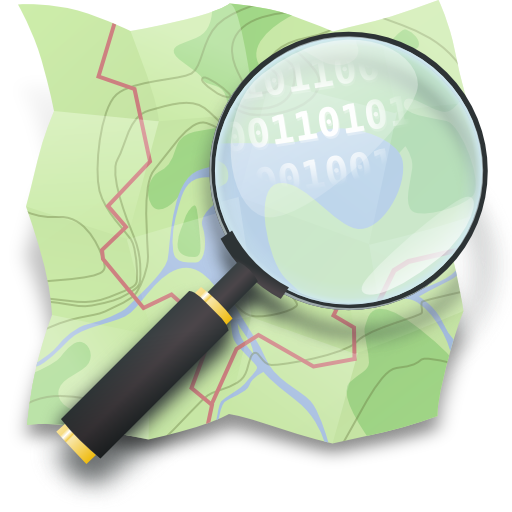
\includegraphics[width=5em]{osm_logo.png}

Besuchen Sie die Website \href{http://www.openstreetmap.org}{http://www.openstreetmap.org}, auf der Sie weltweit verteilte Geodaten finden. Sollten Sie sich registrieren, erlauben Sie dadurch anderen Nutzern, Ihre erstellten Daten unter der ODbL (Open Database License) weiterzuverwenden. Unter \href{http://wiki.openstreetmap.org/wiki/Main\_Page}{http://wiki.openstreetmap.org/wiki/Main\_Page} finden Sie auch eine detaillierte Dokumentation über das Projekt.
\setbox0\vbox{
\begin{minipage}{0.95\linewidth}
\textbf{Aufgabe 1}

\medskip


Untersuchen Sie die beiden oben genannten Websites und beschreiben Sie Ihre Erfahrungen, wobei Ihnen die folgenden Fragen als Richtlinie dienen sollen.
\begin{itemize}
\item {} 
Wie gestaltet sich der Zugang zur Website?

\item {} 
Wie beurteilen Sie das User Interface?

\item {} 
Welchen Nutzungsbedingungen unterliegen die Daten?

\item {} 
Woher kommen die Daten?

\item {} 
Wer haftet für die Daten?

\item {} 
Gibt es einen urheberrechtlichen Schutz?

\item {} 
Wie können die Daten weiterverwendet werden?

\end{itemize}
\end{minipage}}
\begin{center}\setlength{\fboxsep}{5pt}\shadowbox{\box0}\end{center}


\section{Abgabe}
\label{uebung1:abgabe}
Die Abgabe erfolgt über die TUWEL Plattform. Bitte Verwenden Sie das \emph{pdf} Format für Ihre Abgabe. Der Bericht sollte bei einer \textbf{Schriftgröße von 12pt} und einem \textbf{Zeilenabstand von 1.5 Zeilen} ungefähr \textbf{zwei Seiten} umfassen. Als Ergänzung können Sie auch Screenshots in den Text einfügen.


\chapter{Übung 2: Rasterdaten}
\label{uebung2::doc}\label{uebung2:ubung-2-rasterdaten}

\section{Installation}
\label{uebung2:installation}
Für die Durchführung der Übung wird die frei verfügbare OpenSource GIS Software \textbf{QGIS} benutzt. Viele Funktionen von QGIS werden über Plugins bereitgestellt.
\begin{figure}[htbp]
\centering
\capstart


\includegraphics[width=25em]{qgis-splash.png}
\caption{Der Startbildschirm der verwendeten QGIS Version 2.6}\label{uebung2:figqgissplash}\end{figure}

Sollten Sie eine der verwendeten Funktionen nicht finden, sehen Sie im QGIS Menü \emph{Erweiterungen} -\textgreater{} \emph{Erweiterungen verwalten und installieren} nach, ob die entsprechende Funktion installiert und aktiviert ist.

Es wird empfohlen, die Übungen an einem der Rechner im GIS-Lab am Institut zu absolvieren. Es ist jedoch auch möglich, sich die Software auf dem eigenen Computer zu installieren.
Wenn Sie für die Übung angemeldet sind, bekommen Sie automatisch einen Account am Institutsserver zugewiesen. QGIS ist auf diesem Account bereits installiert.


\subsection{Zugang mit dem eigenen Rechner}
\label{uebung2:zugang-mit-dem-eigenen-rechner}
Sie können auch von zu Hause aus über einen Clienten auf Ihrem Account im GIS Labor bearbeiten. Die Client-Software ist unter \href{http://www.x2go.org}{http://www.x2go.org} downloadbar.
Nach der Installation öffnen Sie zur Konfiguration des Clienten in dessen Menü die \textbf{Session preferences} und geben im Tab \textbf{Session} die folgenden Einstellungen ein:
\begin{itemize}
\item {} 
Host: \code{gi30.geoinfo.tuwien.ac.at}

\item {} 
Login: \textless{}Ihr Benutzername\textgreater{}

\item {} 
SSH port: \code{22}

\item {} 
Session type: \code{Custom desktop}

\item {} 
Command: \code{/usr/bin/startxfce4}

\end{itemize}

Im Tab \textbf{Settings}:
\begin{itemize}
\item {} 
Keyboard layout: \code{de}

\item {} 
Keyboard model: \code{pc105/de}

\end{itemize}

Nachdem Sie die Einstellungen bestätigt haben, können Sie die Session mit Ihrem Benutzernamen und Passwort starten.


\subsection{QGIS auf dem eigenen Rechner}
\label{uebung2:qgis-auf-dem-eigenen-rechner}
Sollten Sie QGIS auf Ihrem Computer installieren wollen, finden Sie unter der Adresse \href{http://www.qgis.org}{http://www.qgis.org} im Bereich Download die Dateien für die Installation von QGIS auf Linux, Mac OS X und Windows.


\section{Daten}
\label{uebung2:daten}
Die Daten finden Sie im TUWEL-Kurs zur Übung. Sollten Sie im GIS-Lab oder über den x2go-Client arbeiten, verwenden Sie am besten den Firefox Browser und laden sich die Daten in ein eigenes Verzeichnis.

Wir werden in dieser Übungseinheit hauptsächlich mit \textbf{Rasterdaten} (Abbildung \hyperref[uebung2:figrasterlayer]{ \ref*{uebung2:figrasterlayer}}) arbeiten.
\begin{figure}[htbp]
\centering
\capstart

\scalebox{0.700000}{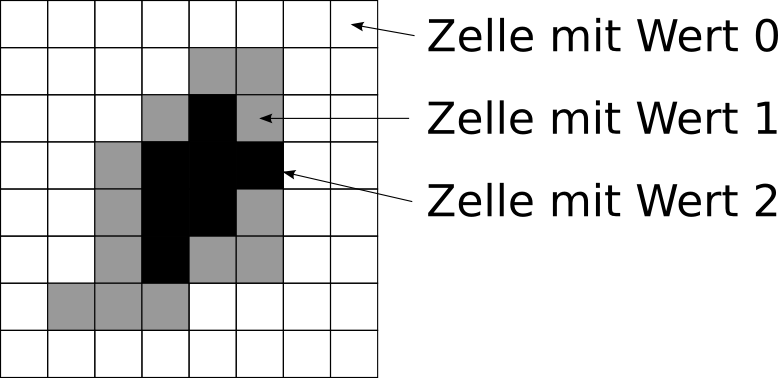
\includegraphics{rasterlayer.png}}
\caption{Der prinzipielle Aufbau eines Rasterlayers}\label{uebung2:figrasterlayer}\end{figure}

Ein Rasterlayer ähnelt einem digitalen Photo. Wenn man weit genug hineinzoomt kann man die \textbf{einzelnen Zellen} erkennen, aus denen sich ein Raster zusammensetzt. Jede Zelle besitzt einen bestimmten Wert. Der gesamte Rasterlayer kann unterschiedlich eingefärbt werden oder auch nur Graustufen besitzen.


\section{Start}
\label{uebung2:start}
Sollten Sie im \textbf{GIS-Lab} oder über den \textbf{x2go-Client} arbeiten, finden sie QGIS im \emph{Applications Menu} unter \emph{Education} -\textgreater{} \emph{QGIS Desktop} (siehe Abbildung \hyperref[uebung2:figserver]{Abbildung  \ref*{uebung2:figserver}}).
\begin{figure}[htbp]
\centering
\capstart

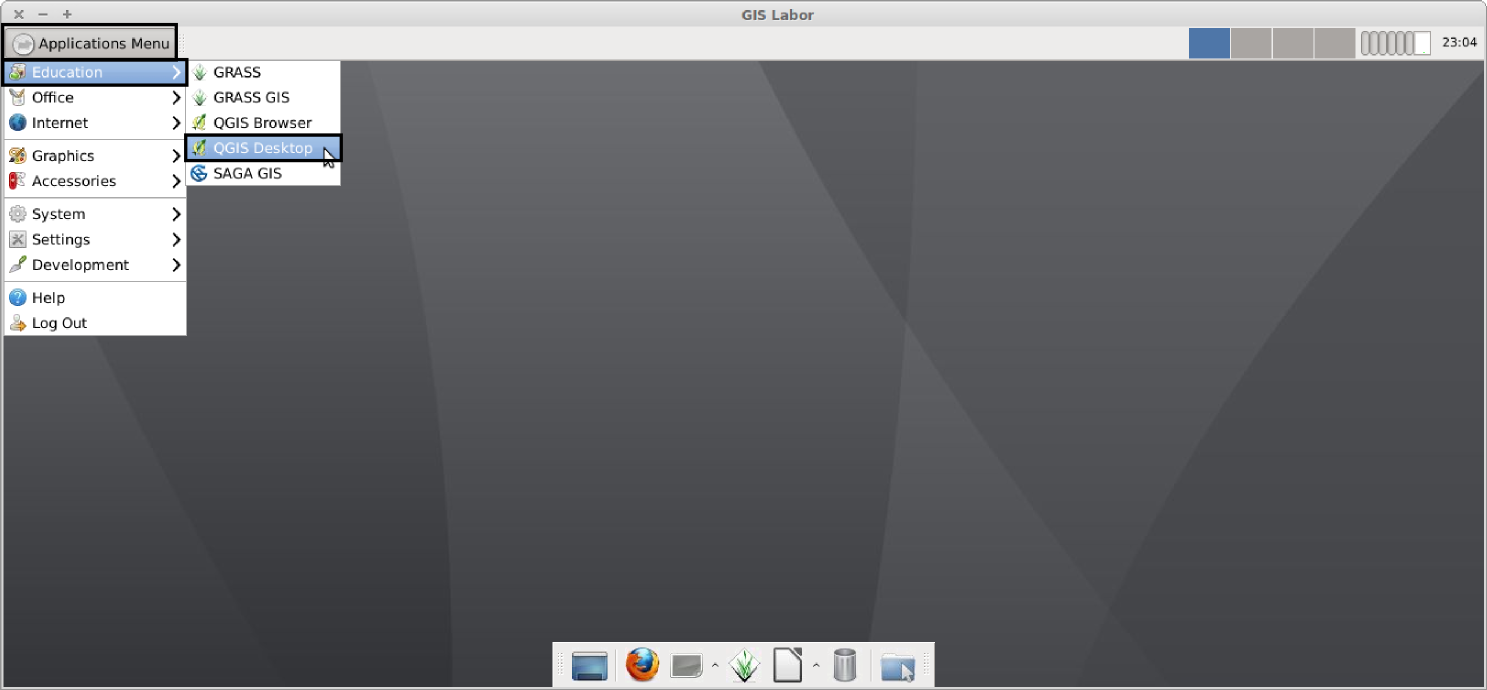
\includegraphics{server_desktop.png}
\caption{Desktopumgebung im GIS-Lab}\label{uebung2:figserver}\end{figure}

Alternativ können Sie auch den Kommandozeilenbefehl \emph{qgis} verwenden, um QGIS zu starten.


\section{Quellen von Geodaten}
\label{uebung2:quellen-von-geodaten}
Mit QGIS können wir \textbf{Daten direkt aus jedem beliebigen Verzeichnis} öffnen. Der Übersicht halber ist es jedoch ratsam, alle Daten, welche zu einem Projekt gehören, in einem einzelnen Verzeichnis zusammen zu speichern.
Dabei kann verschiedene Unterverzeichnisse erstellen um beispielsweise Rasterdaten und Vektordaten zu trennen.

Bei \textbf{größeren Projekten} ist es üblich, dass die Geodaten in einem speziellen \textbf{Datenbanksystem} gespeichert werden. Das hat unter anderem den Vorteil, dass der Zugriff auf die Daten schneller erfolgt oder Zugangsbeschränkungen eingerichtet werden können. QGIS kann auch solche Datenbanken öffnen.

Eine weitere wichtige Ressource für Geodaten sind \textbf{online Dienste} (WFS, WMS, etc ...). Nach Angabe einer URL wird eine Liste aller dort verfügbaren Geodaten angezeigt. Man kann nun auswählen, welche Daten man laden möchte. Der Zugriff auf diese Quellen ist mit QGIS ebenfalls möglich.

Einige wenige Datensätze, welche keine Geodaten im eigentlichen Sinn sind, können ebenfalls von QGIS geöffnet werden. Dazu zählen beispielsweise Tabellen.


\section{Ein neues Projekt}
\label{uebung2:ein-neues-projekt}
QGIS besteht aus einem einzigen Programmfenster mit \textbf{Menüleiste}, mehreren \textbf{Symbolleisten}, einer \textbf{Kartenanzeige} und verschiedenen \textbf{Andockfenstern}.
Sobald das Programm gestartet wurde, wird automatisch ein neues, leeres QGIS Projekt erzeugt.


\section{Koordinatensystem einstellen}
\label{uebung2:koordinatensystem-einstellen}
Bevor wir Daten laden, sollten wir ein \textbf{Koordinatensystem für das gesamte Projekt} definieren. Falls wir dies nicht tun, wird QGIS auf die Standardeinstellung zurückfallen und annehmen, dass alle Daten, welche wir laden werden, im gleichen Koordinatensystem liegen. In vielen Fällen ist diese Annahme korrekt, doch ist es klug, dennoch immer explizit das benutzte Koordinatensystem anzugeben.
\begin{figure}[htbp]
\centering
\capstart

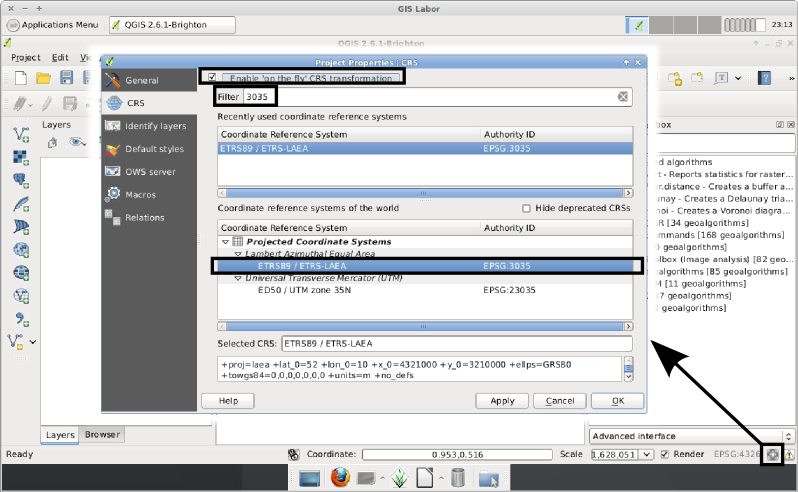
\includegraphics{qgis_srs.png}
\caption{Einstellen eines Koordinatensystems für das gesamte Projekt}\label{uebung2:figsrs}\end{figure}

Um das Koordinatensystem des gesamten Projekts zu definieren, klicken wir auf das \textbf{Icon rechts unten im QGIS Programmfenster} (siehe Abbildung \hyperref[uebung2:figsrs]{ \ref*{uebung2:figsrs}}). Daraufhin öffnet sich das Fenster mit dem Titel \emph{Project Properties \textbar{} CRS (Projekteigenschaften \textbar{} KBS)}.
Zunächst sollten Sie sicherstellen, dass die Option \emph{Enable `on the fly' CRS transformation (Spontan-KBS-Transformation aktivieren)} \textbf{aktiviert} ist. Nur dann wird QGIS (nur für die Anzeige) alle anderen Daten in das Kooridinatensystem umrechnen, welches wir nun einstellen.
In diesem Fenster geben wir im Feld \emph{Filter} die \textbf{EPSG Nummer} \code{3035} ein \footnote{
Der EPSG Code dient zur Identifikation des Koordinatensystems. Das ETRS89 Koordinatensystem hat den Code 3035. Unter \href{http://spatialreference.org/ref/epsg/3035/}{http://spatialreference.org/ref/epsg/3035/} finden Sie eine genauere Beschreibung der Parameter.
}. Dies bewirkt, dass in der Liste mit verfügbaren Koordinatensystemen nur mehr jenes angezeigt wird, welches die EPSG Nummer 3035 besitzt.
Dieses trägt auch den Namen \emph{ETRS89 / ETRS-LAEA}, welches wir auswählen. Danach bestätigen wir diese Auswahl mit dem \emph{OK} Knopf unten rechts.


\section{Daten und Metadaten}
\label{uebung2:daten-und-metadaten}
Um in QGIS Geodaten zu öffnen, kann man entweder auf ein dem Datentyp entsprechendes \textbf{Icon in der Symbolleiste} klicken, oder das \textbf{{}`Browser{}` Fenster} nutzen (siehe Abbildung \hyperref[uebung2:figload]{ \ref*{uebung2:figload}}), um ähnlich wie in einem Dateimanager durch die Verzeichnissen auf dem Computer zu navigieren.
\begin{figure}[htbp]
\centering
\capstart

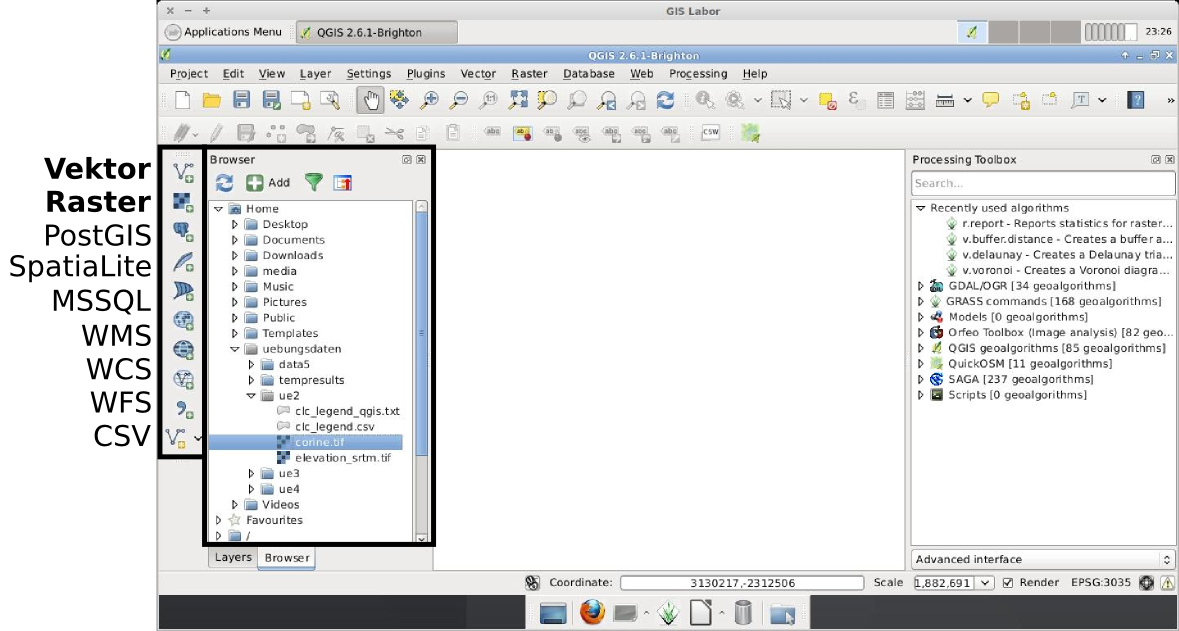
\includegraphics{qgis_data.png}
\caption{Möglichkeiten, Daten zu laden}\label{uebung2:figload}\end{figure}

Als ersten Schritt \textbf{öffnen wir die Datei {}`{}`elevation\_srtm.tif{}`{}`}. Dazu doppelklicken wir auf die Datei im \emph{Browser} Fenster oder öffnen den \emph{Add Raster Layer (Rasterlayer Hinzufügen)} Dialog (zweites Icon von oben in der gelb markierten Symbolleiste in Abbildung \hyperref[uebung2:figload]{ \ref*{uebung2:figload}}).
Es ist auch möglich die Datei aus einem Dateibrowser heraus direkt auf das QGIS Fenster zu ziehen.

Das Programmfenster zeigt nun die soeben geladene Datei im Kartenfenster in der Mitte (Abbildung 3.6).
\begin{figure}[htbp]
\centering
\capstart

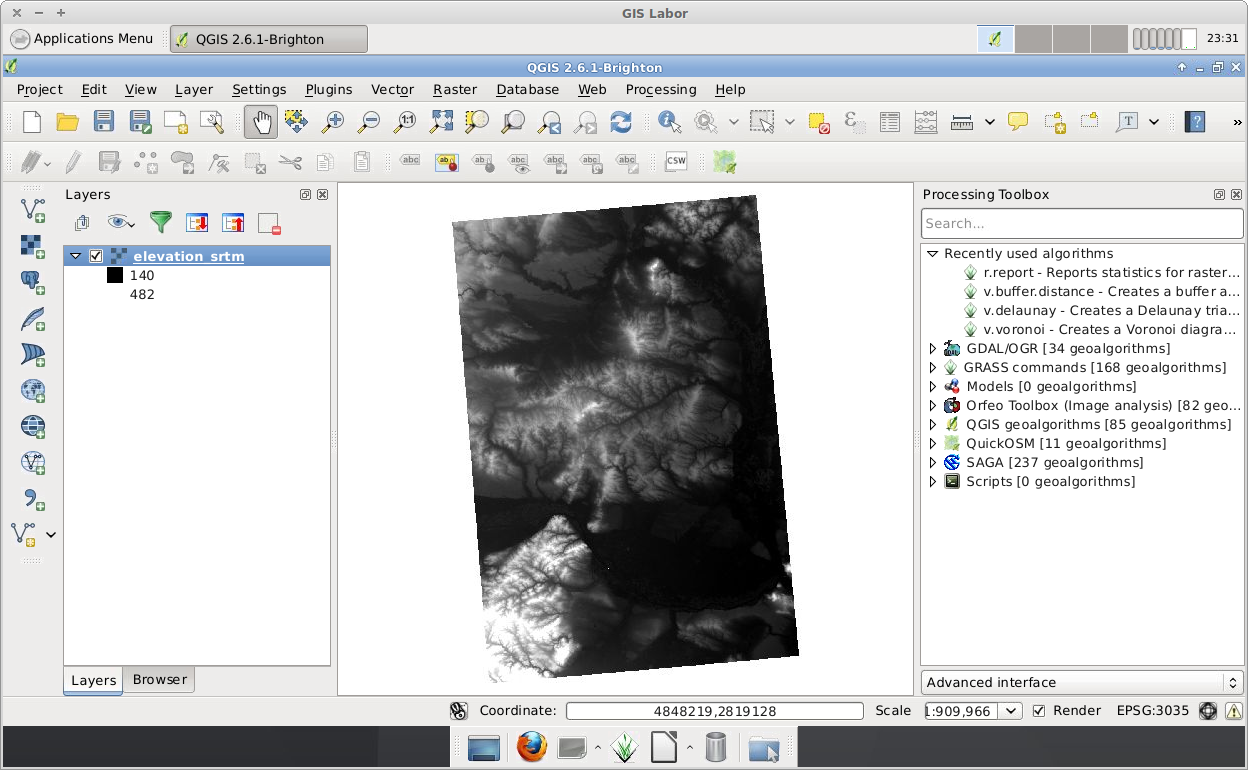
\includegraphics{qgis_srtm.png}
\caption{Die Datei elevation\_srtm.tif in QGIS}\label{uebung2:figsrtm}\end{figure}

Die Datei \code{elevation\_srtm.tif} beinhält \textbf{Höhenwerte} der NASA Shuttle Radar Topography Mission (SRTM) \footnote{
Unter \href{http://dds.cr.usgs.gov/srtm/version2\_1/SRTM3/Eurasia/}{http://dds.cr.usgs.gov/srtm/version2\_1/SRTM3/Eurasia/} stehen Höhendaten mit nahezu globaler Abdeckung zum Download zu Verfügung. Die Höhendaten für diese Übung sind in der Datei N48E016.hgt.zip.
}.
Alle in QGIS geöffneten Daten werden als \emph{Layer} bezeichnet. Wenn mehrere Datensätze gleichzeitig geladen sind, werden diese einzelnen Layer übereinander gelegt. Diese Layer kann man einzeln ein- und ausschalten oder auch deren Reihenfolge ändern. Dies geschiet in der \emph{Layers} Ansicht (das Fenster rechts in Abbildung 3.6).

Um die \textbf{Metadaten} zu einem einzelnen Layer anzusehen, kann man eine Funktion des \emph{Properties (Eigenschaften)} Fensters nutzen. Dieses \textbf{Eigenschaftsfenster für einen Layer} öffnet man, indem man mit der \textbf{rechten Maustaste} darauf klickt und im daraufhin erscheinenen Menü auf \emph{Properties (Eigenschaften)} klickt (siehe Abbildung ).
\begin{figure}[htbp]
\centering
\capstart

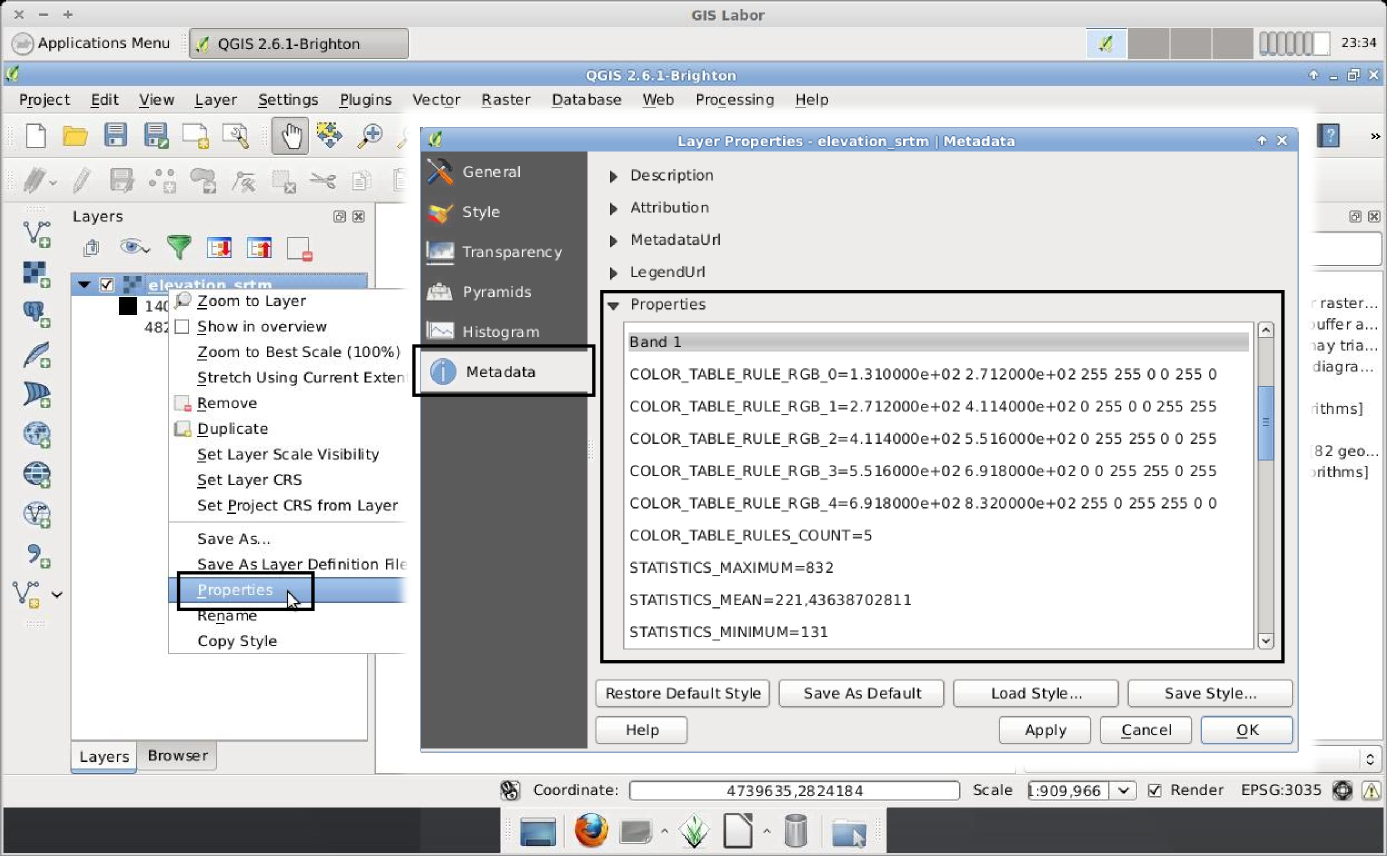
\includegraphics{qgis_properties.png}
\caption{Das Eigenschaftsfenster eines Rasterdatensatzes}\label{uebung2:figsprop}\end{figure}

In diesem Eigenschaftsfenster klicken wir auf den Punkt \emph{Metadata}. Unter dem Abschnitt \emph{Properties (Eigenschaften)} werden eine \textbf{Vielzahl allgemeiner Informationen} angezeigt.
\setbox0\vbox{
\begin{minipage}{0.95\linewidth}
\textbf{Aufgabe 2}

\medskip


Beantworten Sie mit Hilfe der Metadaten des SRTM Layers folgende Fragen:
\begin{itemize}
\item {} 
Wieviele Kanäle (auf Englisch \emph{Band} genannt) besitzt dieser Layer?

\item {} 
Finden Sie die minimalen und maximalen Höhenwerte.

\item {} 
Mit welchem Datentyp sind die Werte im Layer gespeichert?

\end{itemize}

Für diese Aufgabe müssen Sie keinen Screenshot abgeben.
\end{minipage}}
\begin{center}\setlength{\fboxsep}{5pt}\shadowbox{\box0}\end{center}


\section{Verändern der Anzeige}
\label{uebung2:verandern-der-anzeige}
Die Kartenanzeige kann \textbf{verschoben} werden und man kann \textbf{hinein- oder hinauszoomen}.  Solange die Funktion \emph{Pan Map} (siehe Abbildung \hyperref[uebung2:figsmove]{ \ref*{uebung2:figsmove}}) aktiv ist, kann mit der Maus das Kartenfenster verschoben werden. Auch wenn diese Funktion gerade nicht aktiv ist, kann man durch Klicken und Halten der \textbf{mittleren Maustaste} den gleichen Effekt erzielen.
\begin{figure}[htbp]
\centering
\capstart

\scalebox{1.000000}{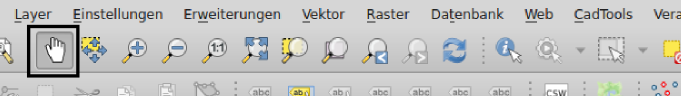
\includegraphics{qgis_menu_move.png}}
\caption{Symbolknopf für die Funktion \emph{Pan Map (Karte verschieben)}}\label{uebung2:figsmove}\end{figure}

Gezoomt kann im einfachsten Fall mit dem \textbf{Mausrad} werden. Falls man einmal den Bezug verlieren sollte und nicht mehr zur Ansicht der geladenen Daten zurückfindet, kann man mit dem Knopf \emph{Zoom Full} (siehe Abbildung \hyperref[uebung2:figsausdehnung]{ \ref*{uebung2:figsausdehnung}}) auf alle gerade geladenen Daten zoomen.
\begin{figure}[htbp]
\centering
\capstart

\scalebox{1.000000}{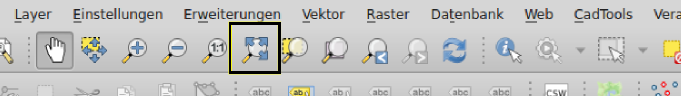
\includegraphics{qgis_ausdehnung.png}}
\caption{Symbolknopf für die Funktion \emph{Zoom Full (Volle Ausdehnung)}}\label{uebung2:figsausdehnung}\end{figure}
\setbox0\vbox{
\begin{minipage}{0.95\linewidth}
\textbf{Aufgabe 3}

\medskip

\begin{itemize}
\item {} 
Stellen Sie sicher, dass die SRTM Höhenkarte geladen ist und zoomen Sie in einen beliebigen Bereich hinein. Speichern Sie diese Ansicht mit der Funktion \emph{Bild speichern als...}, welche Sie im Menüpunkt \emph{Projekt} finden.

\end{itemize}
\end{minipage}}
\begin{center}\setlength{\fboxsep}{5pt}\shadowbox{\box0}\end{center}

Mit der Abfragefunktion \emph{Identify Features} (siehe Abbildung \hyperref[uebung2:figsinfo]{ \ref*{uebung2:figsinfo}}) lässt sich mit einem Mausklick der Wert der Höhenkarte an der Position des Mausklicks anzeigen.
So kann mit nur einem Mausklick die \textbf{Höhe jeder Position der Karte} ermittelt werden.
\begin{figure}[htbp]
\centering
\capstart

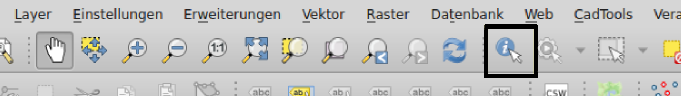
\includegraphics{qgis_info.png}
\caption{Symbolknopf für die Funktion \emph{Identify Features (Objekte Abfragen)}}\label{uebung2:figsinfo}\end{figure}


\section{Farbtabellen}
\label{uebung2:farbtabellen}
Wir laden nun einen weiteren Datensatz aus der Datei \emph{corine.tif} in das QGIS Projekt. Diese \textbf{Corine Land Cover Classification} wird von der European Environment Agency \footnote{
www.eea.europa.eu
} bereitgestellt. In der Datei \emph{clc\_legend.csv} kann man eine kurze \textbf{Beschreibung der Landbedeckungsklassen} finden.
Als nächstes wollen wir diese Beschreibungen zu den Klassennummern der Rasterdatei hinzufügen. Erfreulicher weise wid speziell für QGIS bereits eine Datei zur Verfügung gestellt, die \textbf{die einzelnen Rasterwerte den Landbedeckungsklassen zuordnet}.
\begin{figure}[htbp]
\centering
\capstart

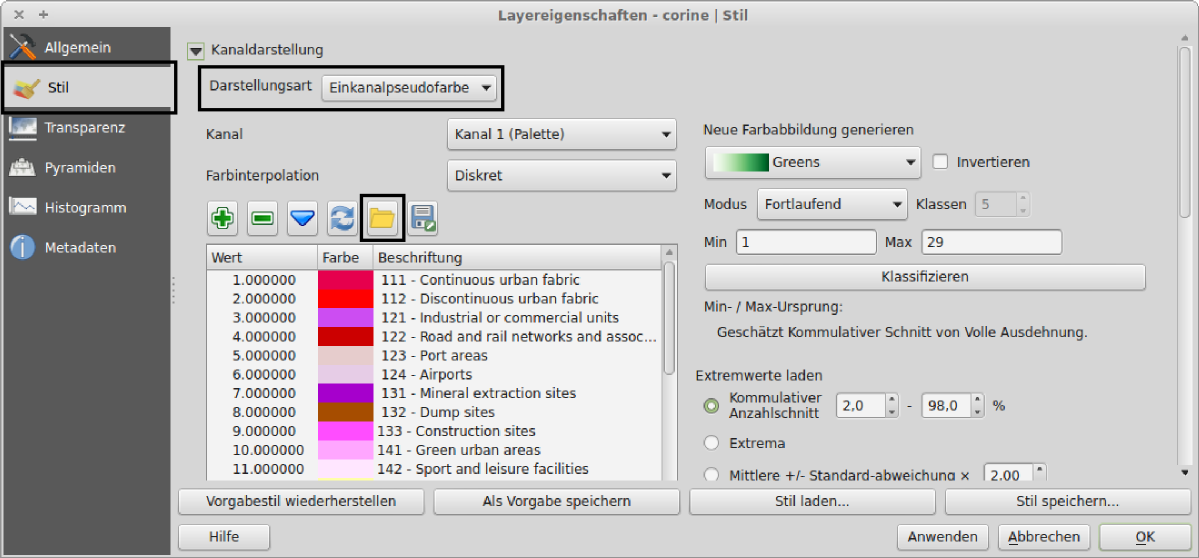
\includegraphics{qgis_farbpalette.png}
\caption{Das Einstellungsfenster zur Konfiguration einer Farbpalette}\label{uebung2:figsfarbpalette}\end{figure}

Um diese \textbf{Datei zu laden}, öffnen wir diesmal das \emph{Properties (Eigenschaften)} Fenster des Corine Layers und gehen auf den Menüpunkt \emph{Style (Stil)} (siehe Abbildung \hyperref[uebung2:figsfarbpalette]{ \ref*{uebung2:figsfarbpalette}}).
Danach ändern wir den \emph{Render type (Darstellungsart)} auf \emph{Singleband pseudocolor (Einkanalpseudofarbe)}. Nun klicken wir auf den Knopf \emph{Load color map from file (Farbabbildung aus Datei laden)} (siehe Markierung in der Abbildung) und wählen die Datei \emph{clc\_legend\_qgis.txt} aus den Übungsdaten aus. Diese Datei beinhält die Zuordnung der Rasterwerte zu den Landbedeckungsklassen.
Nach einem Klick auf \emph{OK}, erscheinen nun \textbf{neben den Farben (Spalte {}`Color (Farbe){}`) der einzelnen Rasterwerte} (Spalte \emph{Value (Wert)}) auch die \textbf{Bezeichnungen der Landbedeckungsklassen (Spalte {}`Label (Beschriftung){}`)}.

Wechseln wir nun zur Ansicht \emph{Histogram} (siehe Abbildung \hyperref[uebung2:figshistogram]{ \ref*{uebung2:figshistogram}}). Hier wird die \textbf{Häufigkeit der einzelnen Rasterwerte} angezeigt. Die \textbf{horizontale Achse} namens \emph{Pixel Value (Pixelwert)} beschreibt die einzelnen Rasterwerte, die \textbf{vertikale Achse} namens \emph{Frequency (Frequenz)} beschreibt die Häufigkeit der einzelnen Rasterwerte.
\begin{figure}[htbp]
\centering
\capstart

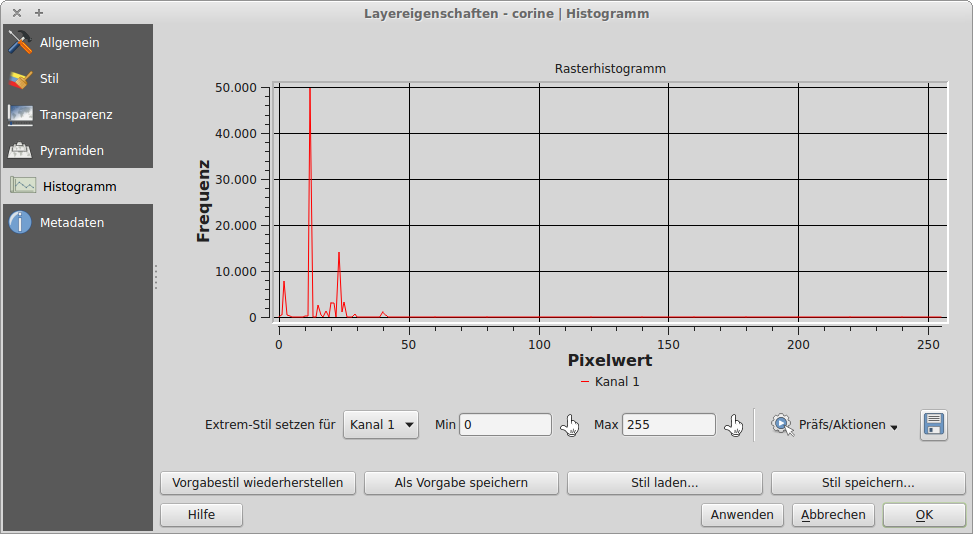
\includegraphics{qgis_histogram.png}
\caption{Das Histogrammfenster}\label{uebung2:figshistogram}\end{figure}
\setbox0\vbox{
\begin{minipage}{0.95\linewidth}
\textbf{Aufgabe 4}

\medskip

\begin{itemize}
\item {} 
Finden sie mithilfe des Histograms den häufigsten Rasterwert (Pixelwert) heraus. Sie können mit der \textbf{Maus in das Histogram hineinzoomen}, um den genauen Wert herauszufinden. Wenn sie den Wert ermittelt haben, welchsen Sie zurück zur \emph{Style} Ansicht und vergleichen den von Ihnen gefundenen Rasterwert mit der zugehörigen Beschriftung. So ermitteln sie den \textbf{Namen der häufigsten Bodenbedeckungsklasse}. Notieren Sie diese.

\end{itemize}

Für diese Aufgabe müssen Sie keinen Screenshot oder Kartenbild abgeben.
\end{minipage}}
\begin{center}\setlength{\fboxsep}{5pt}\shadowbox{\box0}\end{center}


\section{Berechnung von Konturlinien}
\label{uebung2:berechnung-von-konturlinien}
Isolinien verbinden Punkte gleichen Wertes eines kontinuierlichen Feldes. Meistens wird durch das Feld eine physikalische Größe beschrieben. In QGIS kann man Isolinien mit der Funktion \emph{Contour (Kontur)} berechnen. Man findet diese im Menü \emph{Raster} -\textgreater{} \emph{Extraction}. Der sich nun öffnende Dialog sieht aus wie in Abbildung \hyperref[uebung2:figscontour]{ \ref*{uebung2:figscontour}} dargestellt.
\begin{figure}[htbp]
\centering
\capstart

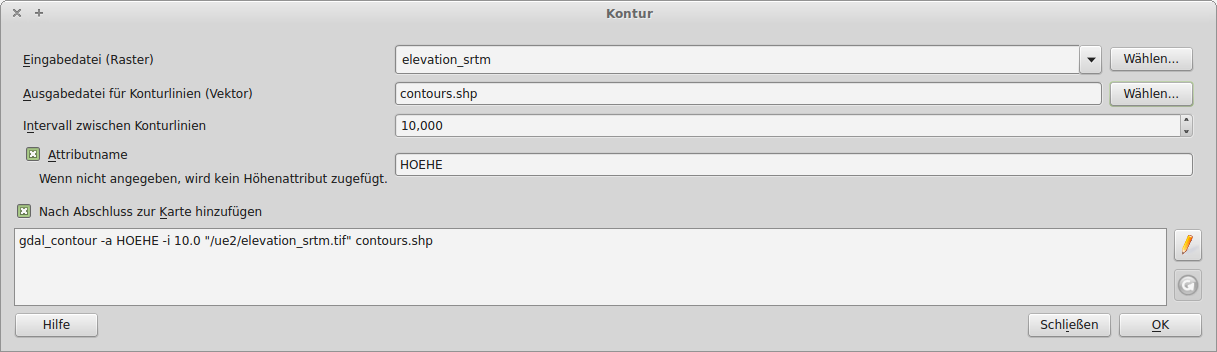
\includegraphics{qgis_contours.png}
\caption{Die Funktion zum Erstellen von Konturlinien}\label{uebung2:figscontour}\end{figure}

Unter dem Feld \emph{Input file (Eingabedatei)} wählen wir unsere \textbf{Höhendaten} namens \emph{elevation\_srtm} aus.
Im Feld \emph{Output file for contour lines (Ausgabedatei für Konturlinien)} geben wir die Datei an, in der die Isolinien \textbf{gespeichert} werden.
Unter \emph{Interval between contour lines (Intervall zwischen Konturlinien)} wird die \textbf{Schrittweite zwischen den einzelnen Konturlinien} angegeben. Die Schrittweite sollte im Allgemeinen \textbf{nicht zu dicht} gewählt werden, um das Gelände nicht zu überdecken, aber auch \textbf{nicht zu weit}, da ansonsten wichtige Informationen über die Variation des Feldes verloren gehen.
Es ist zu empfehlen, die Felder \emph{Attribute name (Attributname)} und \emph{Load into canvas when finished (Nach Abschluss zur Karte hinzufügen)} \textbf{anzuhaken}.
\setbox0\vbox{
\begin{minipage}{0.95\linewidth}
\textbf{Aufgabe 5}

\medskip

\begin{itemize}
\item {} 
Überlegen Sie sich eine geeignete Schrittweite und berechnen Sie Konturlinien aus dem SRTM Höhenraster. Legen Sie die Höhenlinien über die Höhenkarte und speichern Sie die Karte abermals als Bild unter einem aussagekräftigen Namen ab und notieren sie die Schrittweite, die Sie verwendet haben.

\end{itemize}
\end{minipage}}
\begin{center}\setlength{\fboxsep}{5pt}\shadowbox{\box0}\end{center}


\section{Geländeneigung}
\label{uebung2:gelandeneigung}
Als letzten Punkt wollen wir noch die \textbf{Geländeneigung} berechnen. Der Wert \emph{slope} repräsentiert die Geländeneigung am \textbf{Ort einer Zelle}. Die Geländeneigung kann in \textbf{Grad oder in Prozent} berechnet werden. Mit dem Befehl \emph{DEM (Terrain models) (DHM (Geländemodell) )} im Menüpunkt \emph{Raster} -\textgreater{} \emph{Analysis} lässt sich dieser Wert berechnen.

In Abbildung \hyperref[uebung2:figsneigung]{ \ref*{uebung2:figsneigung}} kann man den Dialog zum Erstellen der Neigung sehen. Stellen auch Sie ihn entsprechend ein und definieren Sie einen \emph{Output file (Ausgabedatei)}. Beachten Sie, dass bei manchen Betriebssystemen der Dateiname die \textbf{Endung .tif} haben muss. Ansonsten tritt ein \textbf{Fehler} beim Ausführen der Funktion auf.
\begin{figure}[htbp]
\centering
\capstart

\scalebox{0.500000}{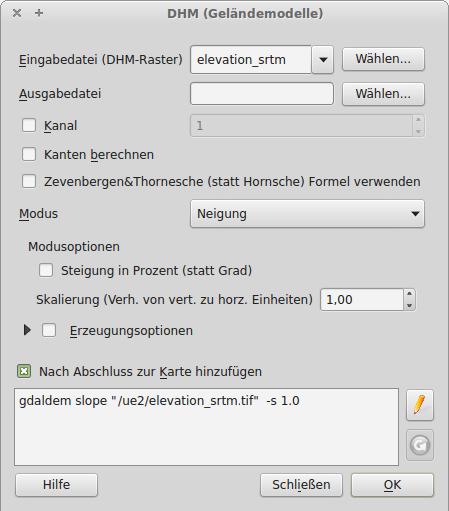
\includegraphics{qgis_neigung.png}}
\caption{Die Funktion zum Berechnen der Neigung}\label{uebung2:figsneigung}\end{figure}

Die Ansicht der Neigungskarte lässt sich noch weiter optimieren. Nehmen wir an, wir sind ausschließlich an Neigungen zwischen 5° und 10° interessiert. Um genau diesen Bereich darzustellen, öffnen wir das \emph{Properties (Eigenschaften)} Fenster des neu erstellen Neigungs-Layers und welchseln auf die \emph{Style (Stil)} Ansicht. Dort setzen wir die Option \emph{Render type (Darstellungsart)} abermals auf den Eintrag \emph{Singleband pseudocolor (Einkanalpseudofarbe)} und \emph{Color interpolation (Farbinterpolation)} auf \emph{Discrete}.

Nun können wir die einzelnen Einträge hinzufügen, um die Neigungsdaten umzufärben. Mit einem Klick auf das \scalebox{0.500000}{
\includegraphics{mActionSignPlus.png}} Symbol wird ein neuer Eintrag hinzugefügt. Die Eigenschaften des neu erzeugten Eintrages können nun verändert werden. Wir belassen die Spalte \emph{Value (Wert)} bei \emph{0}, aber ändern dessen \emph{Color (Farbe)} auf ein einfaches Weiß. Ein weiterer Eintrag sollte den \emph{Wert} \emph{4,999} besitzen und abermals \emph{Weiß} als \emph{Farbe} eingestellt werden. Dies bewirkt, dass alle Werte zwischen \emph{0} und \emph{4,999} als Weiß angezeigt werden. Durch weitere Einträge kann man nun den Bereich zwischen \emph{5} und \emph{10} in einer anderen Farbe darstellen, weitere Werte darüber wieder mit der Farbe \emph{Weiß}.
\setbox0\vbox{
\begin{minipage}{0.95\linewidth}
\textbf{Aufgabe 6}

\medskip

\begin{itemize}
\item {} 
Berechnen Sie die Neigung

\item {} 
Passen Sie den Stil des Neigungsdatensatzes wie oben beschrieben an

\item {} 
Speichern Sie die Ansicht der Neigungkarte als Bild unter einem aussagekräftigen Namen.

\end{itemize}
\end{minipage}}
\begin{center}\setlength{\fboxsep}{5pt}\shadowbox{\box0}\end{center}


\section{Speichern des Projekts}
\label{uebung2:speichern-des-projekts}
Sie können das QGIS Projekt mit dem Menüeintrag \emph{Project} -\textgreater{} \emph{Save as... (Speichern als...)} abspeichern. Bedenken Sie hierbei, dass innerhalb einer Projektdatei nur die Zusammenstellung und das Aussehen der einzelnen Layer gespeichert wird. Die Datensätze selber sind in ihren eigenen Dateien gespeichert. Wenn Sie also ein QGIS Projekt kopieren und weitergeben möchten, müssen sie neben der QGIS Projektdatei auch die Datensätze selber kopieren.


\section{Abgabe}
\label{uebung2:abgabe}
Beantworten Sie die Fragen im Text und fügen Sie alle gespeicherten Bilder und Informationen zu einem Dokument zusammen. Geben Sie Ihre fertige Arbeit als pdf in TUWEL ab.


\chapter{Übung 3: Erweiterte Rateroperationen}
\label{uebung3:ubung-3-erweiterte-rateroperationen}\label{uebung3::doc}
Die Stadt Wien stellt unter \href{http://data.wien.gv.at}{http://data.wien.gv.at} im Rahmen der Open Government Data (OGD) Initiative Verwaltungsdaten frei zur Verfügung. Die Daten werden unter anderm auch im World Geodetic System 1984 (WGS84) bereitgestellt.


\section{Transformation von WGS84 nach ETRS89}
\label{uebung3:transformation-von-wgs84-nach-etrs89}
Die Daten der Stadt Wien liegen in einem anderen Koordinatensystem als die SRTM– und Corine–Daten. Mit QGIS stellt dies kein Problem dar. Richtig konfiguriert, werden die Koordinaten der unteschiedlichen Daten (nur für die Anzeige) derart umgerechnet, dass diese zusammenpassen (vergleiche Abbildungen \hyperref[uebung3:figumprojektion2]{ \ref*{uebung3:figumprojektion2}} und \hyperref[uebung3:figumprojektion1]{ \ref*{uebung3:figumprojektion1}}).
\begin{figure}[htbp]
\centering
\capstart

\scalebox{0.800000}{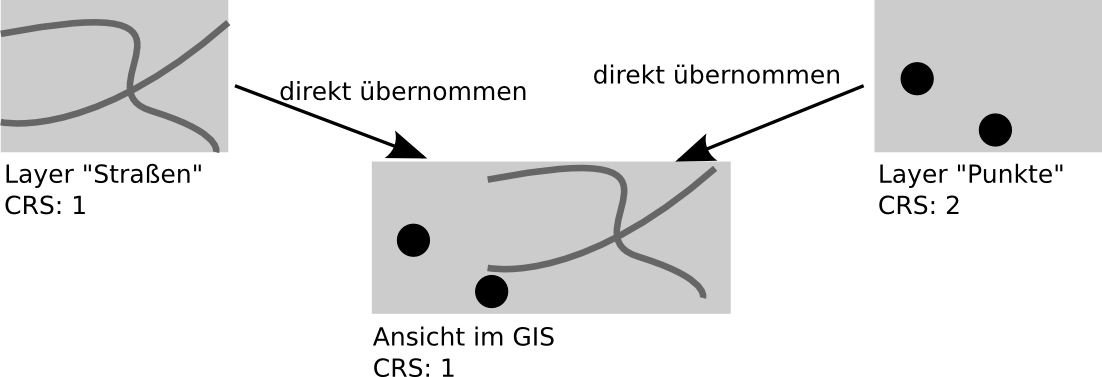
\includegraphics{umprojektion2.png}}
\caption{Wenn Layer unterschiedlicher Koordinatensysteme nicht umprojelziert werden, liegen diese nicht übereinander (die Anzeige im GIS stimmt nicht)}\label{uebung3:figumprojektion2}\end{figure}
\begin{figure}[htbp]
\centering
\capstart

\scalebox{0.800000}{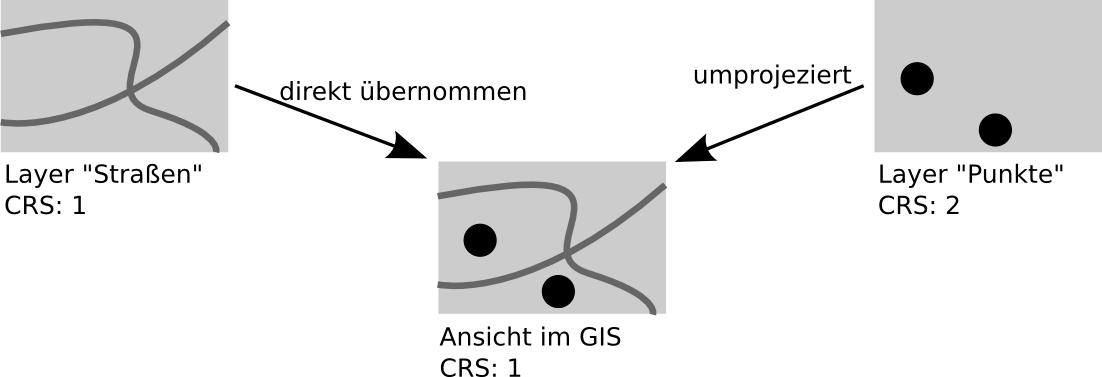
\includegraphics{umprojektion1.png}}
\caption{Wenn Layer unterschiedlicher Koordinatensysteme umprojeziert werden, dann werden diese richtig dargestellt (die Anzeige im GIS stimmt)}\label{uebung3:figumprojektion1}\end{figure}

Dazu müssen Sie sicherstellen, dass (wie im vorherigen Aufgabenblatt in \emph{koordinatensystem}) ein eindeutiges Koordinatensystem für das gesamte Projekt eingestellt ist. QGIS übernimmt nun den Rest und rechnet die Koordinatensysteme aller Layer in jenes des gesamten Projekts um.

Wenn man Berechnungen mit diesen Daten anstellen will ist es jedoch notwendig, dass diese im gleichen Koordinatensystem vorliegen. Ansonsten kommt es zu fehlerhaften Ergebnissen. Zu diesem Zweck können wir diese umprojeziert abspeichern. Die zuvor beschriebene automatische Umprojektion betrifft nur die Anzeige der Daten.
Mit einem Rechtsklick auf den Eintrag des geladenen Layers in der Layeransicht (rechts von der Kartenanzeige in GIS), kann im sich öffnenden Kontextmenü der Eintrag \emph{Save As (Speichern Als)} ausgewählt werden. Es öffnet sich ein Einstellungsfenster für den Export des ausgewählten Layers (siehe Abbildung \hyperref[uebung3:figsaveas]{ \ref*{uebung3:figsaveas}}).
In diesem Fenster muss nun der Eintrag für \emph{CRS (KBS)} auf \emph{Selected CRS (Gewähltes KBS)} gesetzt werden, damit wir manuell ein Koordinatensystem auswählen können, in das die Daten, die wir exportieren wollen, umgerechnet werden.
\begin{figure}[htbp]
\centering
\capstart

\scalebox{1.000000}{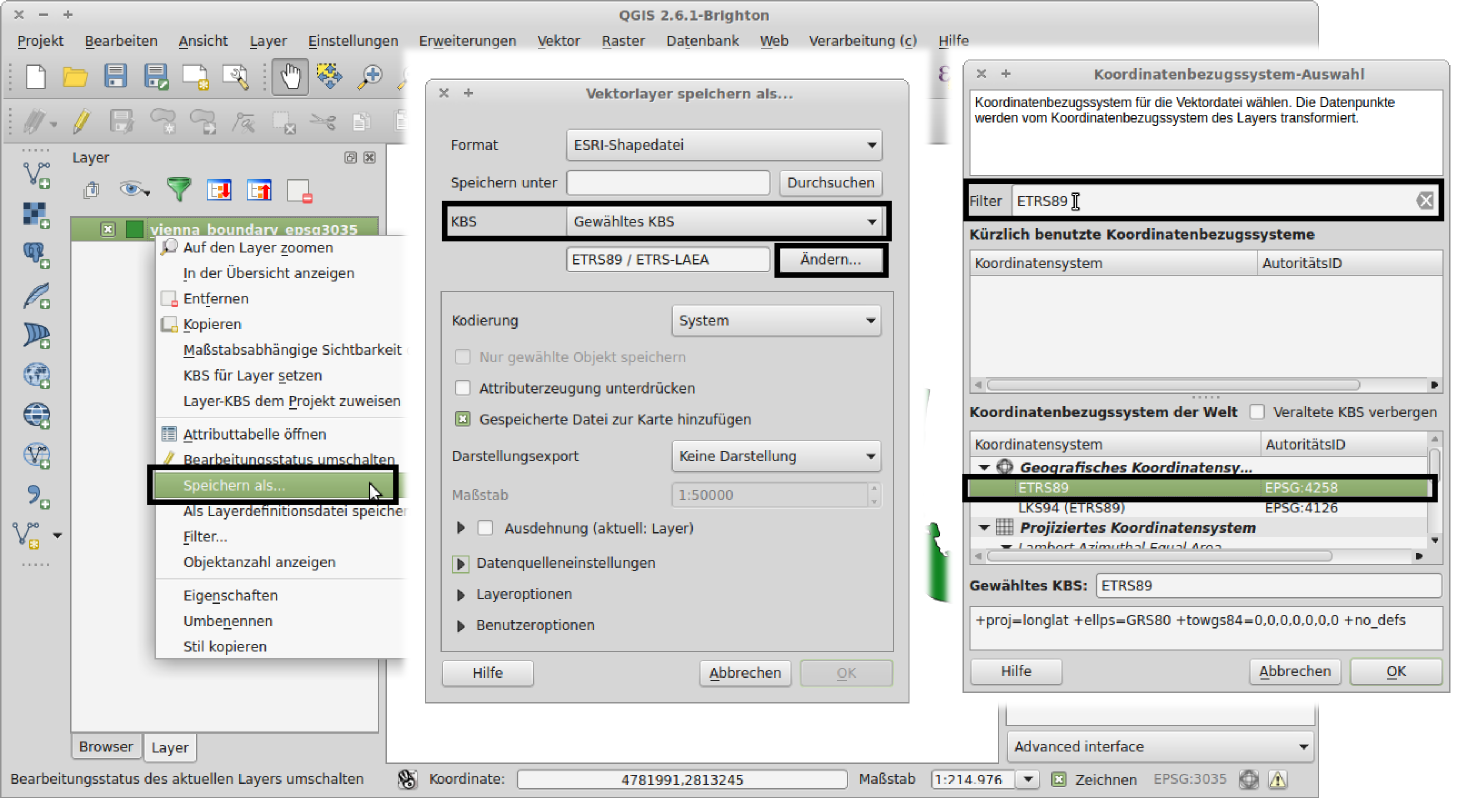
\includegraphics{qgis_saveas.png}}
\caption{Um einen Layer umzuprojezieren, müssen wir diesen mit einem neuen Koordinatensystem exportieren und laden}\label{uebung3:figsaveas}\end{figure}

Suchen Sie nach dem Eintrag \emph{ETRS89}, wählen Sie diesen aus und bestätigen Sie die Auswahl mit dem \emph{OK} Knopf.
Im Feld \emph{Save as (Speichern unter)} muss nun noch ein Dateiname angegeben werden, in die die umprojezierten Daten gespeichert werden sollen.
Wennd das Feld \emph{Gespeicherte Datei zur Karte hinzufügen} angehakt ist, müssen wir keine weiteren Schritte unternehmen, um die exportierten Daten zu laden. Mit einem Klick auf das \emph{OK} Feld werden diese unprojeziert, in die neue Datei gespeichert und diese automatisch in QGIS geladen.
\setbox0\vbox{
\begin{minipage}{0.95\linewidth}
\textbf{Aufgabe 7}

\medskip

\begin{itemize}
\item {} 
Stellen Sie sicher, dass das Koordinatensystem für Ihr Projekt auf ETRS89 eingestellt ist und die \emph{Spontan-KBS-Transformation} aktiviert ist.

\item {} 
Laden Sie den Datensatz \emph{BEZIRKSGRENZENOGD.shp} aus dem entsprechenden Unterverzeichnis der Daten für die Übung 3 in QGIS und speichern Sie diesen umprojeziert in das Koordinatensystem ETRS89 unter einem aussagekräftigen Namen (beispielsweise \emph{bezirksgrenzenogd\_etrs89.shp}) ab. Laden Sie diesen exportierten Layer ebenfalls in QGIS, sofern dies nicht automatisch nach dem Export geschehen ist.

\end{itemize}
\end{minipage}}
\begin{center}\setlength{\fboxsep}{5pt}\shadowbox{\box0}\end{center}


\section{Die Analyse-Toolbox (Processing)}
\label{uebung3:die-analyse-toolbox-processing}
Neben QGIS gibt es eine ganze Reihe weiterer OpenSource GIS Applikationen, welche über Jahre, manche sogar Jahrzehnte hinweg optimiert und verbessert wurden.
Einige nennenswerte Anwendungen dierser Art sind
\begin{itemize}
\item {} 
das \emph{System for Automated Geoscientific Analyses} (SAGA), \href{http://www.saga-gis.org/en/index.html}{http://www.saga-gis.org/en/index.html}

\item {} 
und das \emph{Geographic Resource Analysis Support System} (GRASS GIS), \href{http://grass.osgeo.org/}{http://grass.osgeo.org/}

\end{itemize}
\begin{figure}[htbp]
\centering
\capstart

\scalebox{0.700000}{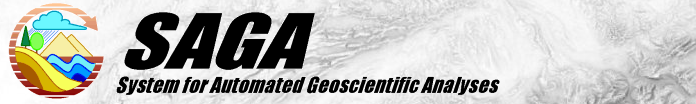
\includegraphics{saga_logo.png}}
\caption{Das Logo von SAGA}\label{uebung3:figsaga}\end{figure}

Insbesondere letzteres hat eine lange Geschichte und gehört zum Urgestein der GIS Welt. Ursprünglich entwickelt von der US Army, wurde es zu einem Zugpferd der OpenSource GIS Community und wird auch heute noch weiterentwickelt. Ein interessantes Werbevideo von 1987 (abrufbar unter \href{https://www.youtube.com/watch?v=U3Hf0qI4JLc}{https://www.youtube.com/watch?v=U3Hf0qI4JLc} ) zeigt den damaligen Entwicklungsstand.
\begin{figure}[htbp]
\centering
\capstart

\scalebox{1.000000}{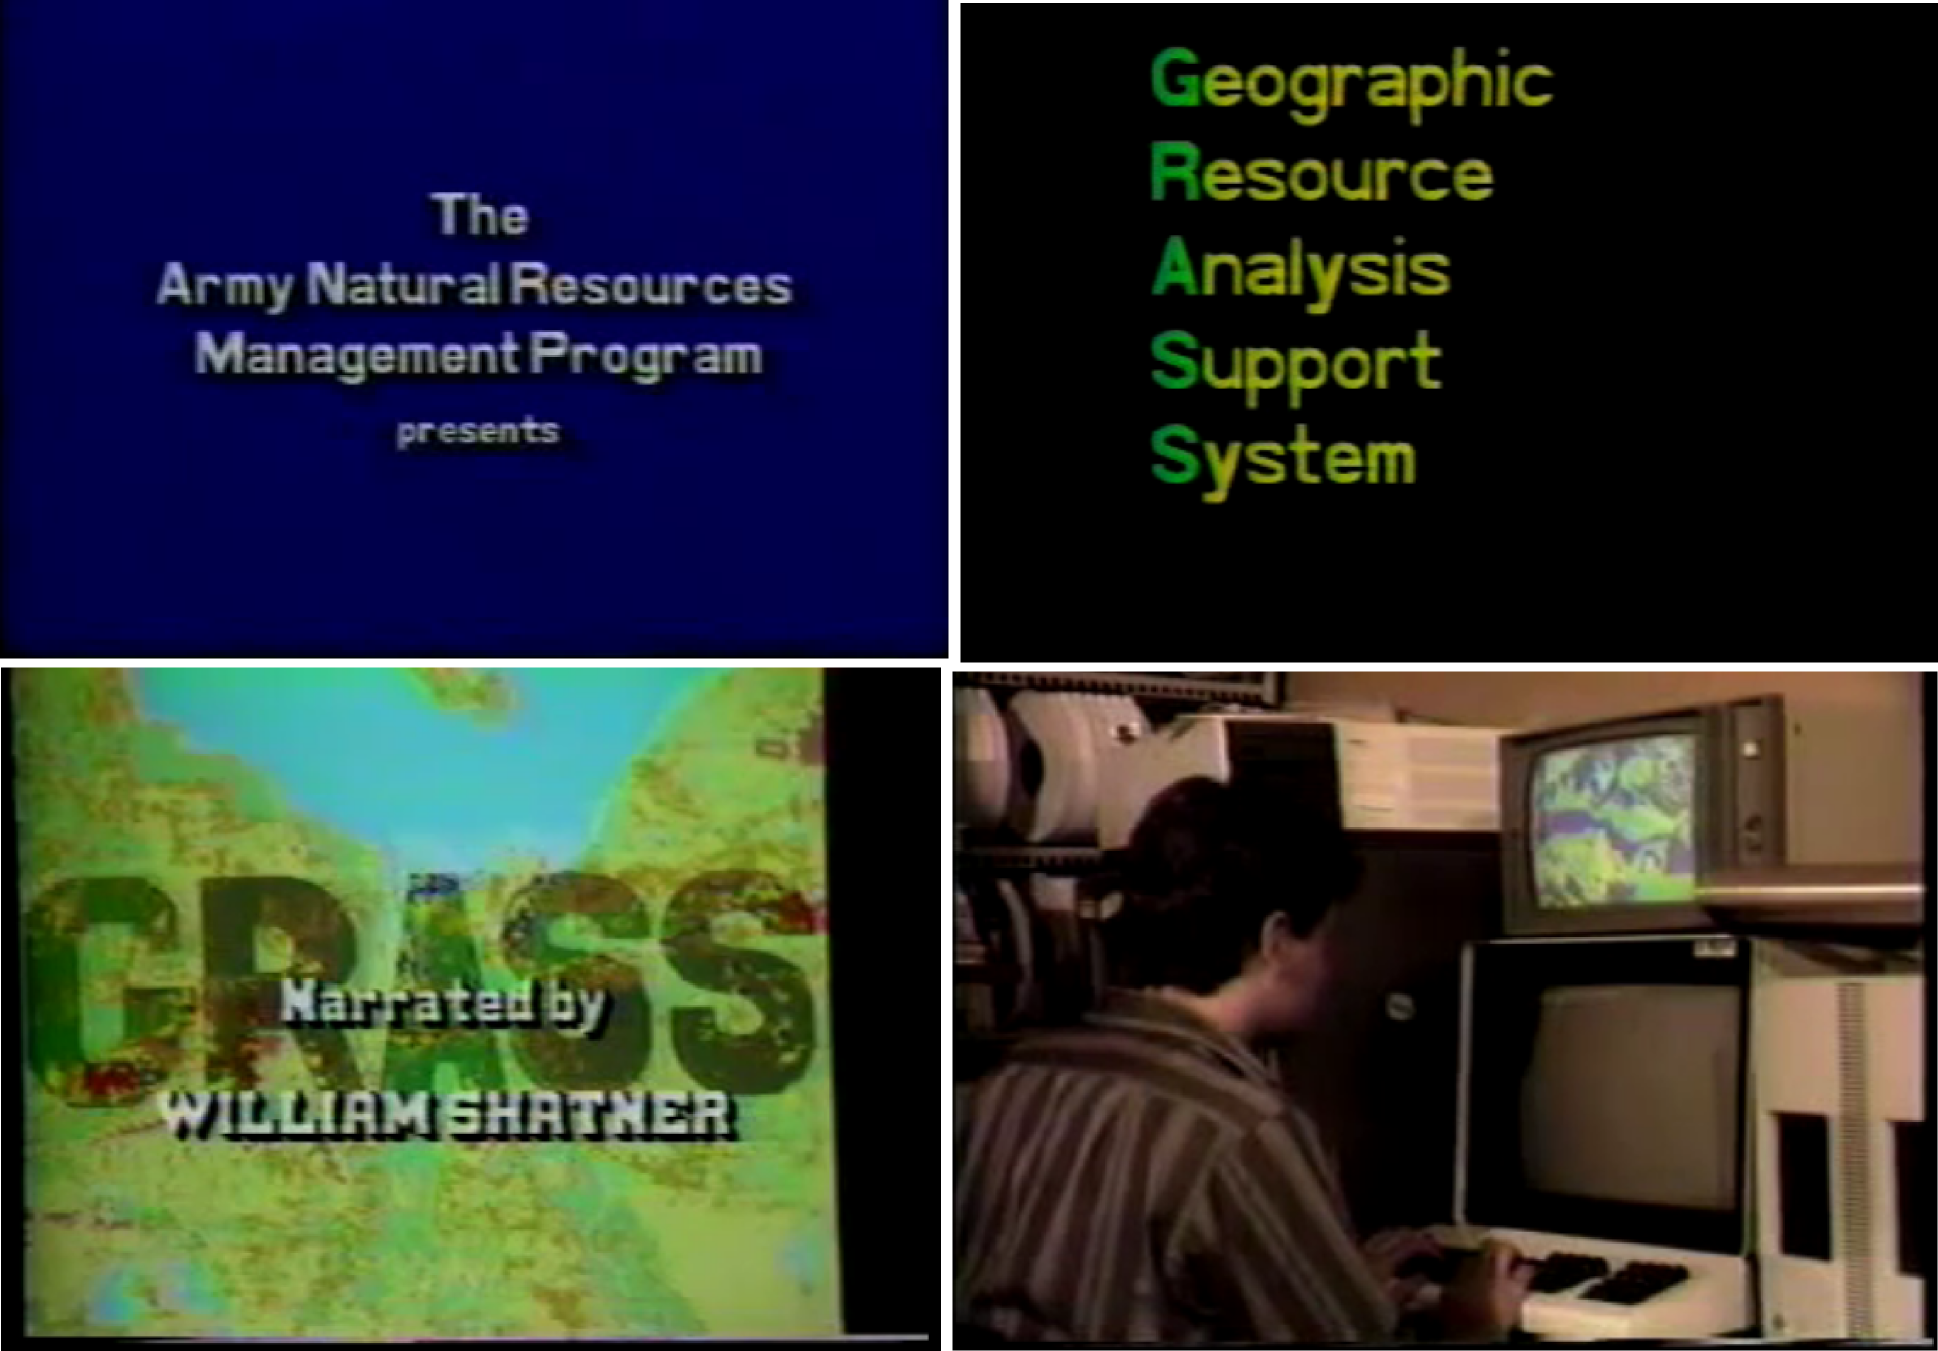
\includegraphics{grass.png}}
\caption{Ausschnitte aus dem GRASS GIS Werbevideo von 1987}\label{uebung3:figgrass}\end{figure}

Um nicht das Rad neu zu erfinden, gibt es in QGIS die Möglichkeit, auf die Algorithmen dieser anderen GIS Anwendungen zurückzugreifen. Dies geschiet mit der so genannten \emph{Processing} Toolbox (auf Deutsch nennt sich diese \emph{Verarbeitung}). In Abbildung \hyperref[uebung3:figprocessing]{ \ref*{uebung3:figprocessing}} ist diese rechts des Kartenfensters zu sehen. Wenn diese nicht angezeigt wird, kann sie über den Menüeintrag \emph{Processing (Verarbeitung)} -\textgreater{} \emph{Toolbox (Werkzeugkiste)} eingeschaltet werden.
\begin{figure}[htbp]
\centering
\capstart

\scalebox{1.000000}{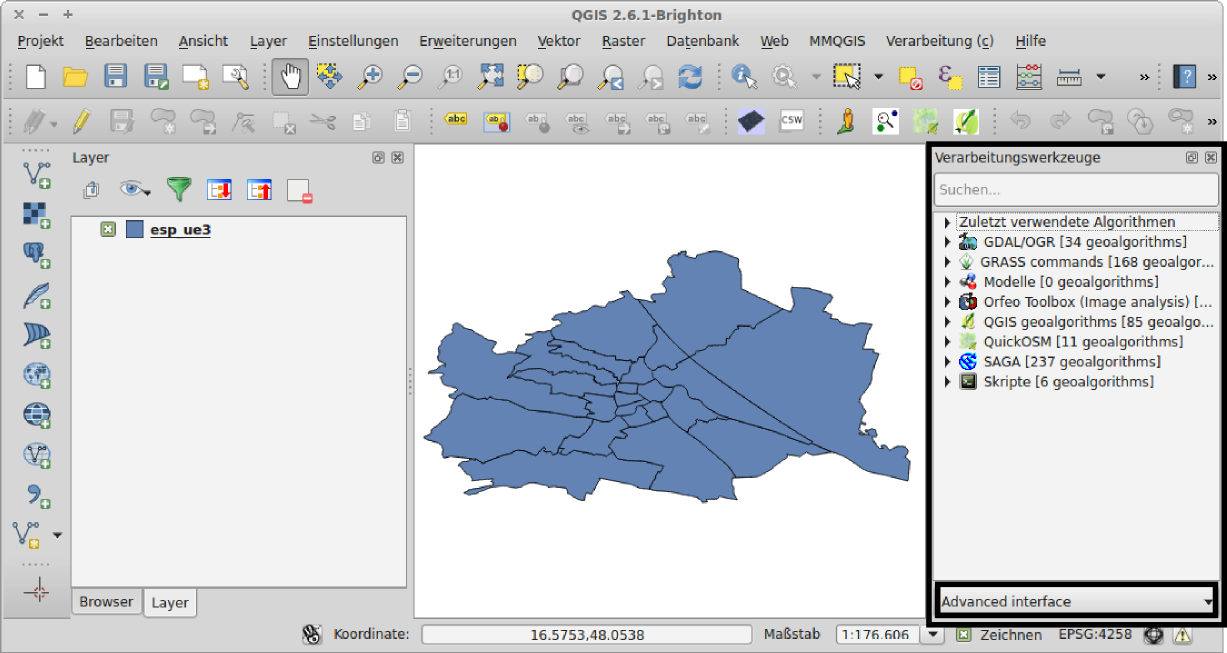
\includegraphics{qgis_processing.png}}
\caption{Die Processing Toolbox in QGIS}\label{uebung3:figprocessing}\end{figure}

Im unteren Bereich kann man mittels einer Auswahlliste zwischen dem \emph{Simplified Interface} und dem \emph{Advanced Interface} wählen. Ich empfehle für Experten, welche wir ja werden wollen, das \emph{Advanced Interface}. Mit diesem können wir erkennen, zu welchem GIS Programm der von uns gewählte Geo-Algorithmus gehört.

Um einen bestimmten Algorithmus auszuwählen, kann man sich entweder durch die Baumstruktur der Processing Toolbox klicken oder man gibt einen Suchbegriff in das Suchfenster im oberen Bereich der Toolbox ein. Dies gestaltet sich als sehr effizient, wenn man bereits weiß, welchen Namen der gewünschte Algorithmus trägt.


\section{Reklassifikation}
\label{uebung3:reklassifikation}
Stellen Sie nun sicher, dass Sie den \textbf{Corine Datensatz} aus Übung 2 geladen haben und die Einkanalpseudofarbenpalette eingestellt ist (ebenfalls wie in Übung 2 beschrieben).
Dieser Corine Raster enthält 44 Landbedeckungsklassen, die wiederum in fünf gröbere Klassen zusammengefasst werden. Die Aufschlüsselung in Klassen samt Beschreibungen kann in der Datei \emph{clc\_legend.csv} nachgelesen werden.

Mit dem Algorithmus mit dem Namen \emph{r.recode} kann der Corine Raster neu klassifiziert werden. Dieser Befehl gehört ursprünglich zu GRASS GIS.
Wenn man diese Funktion mithilfe der \emph{Processing} Toolbox geöffnet hat, zeigt sich das Fenster wie in Abbildung \hyperref[uebung3:figrecode]{ \ref*{uebung3:figrecode}}.
\begin{figure}[htbp]
\centering
\capstart

\scalebox{0.700000}{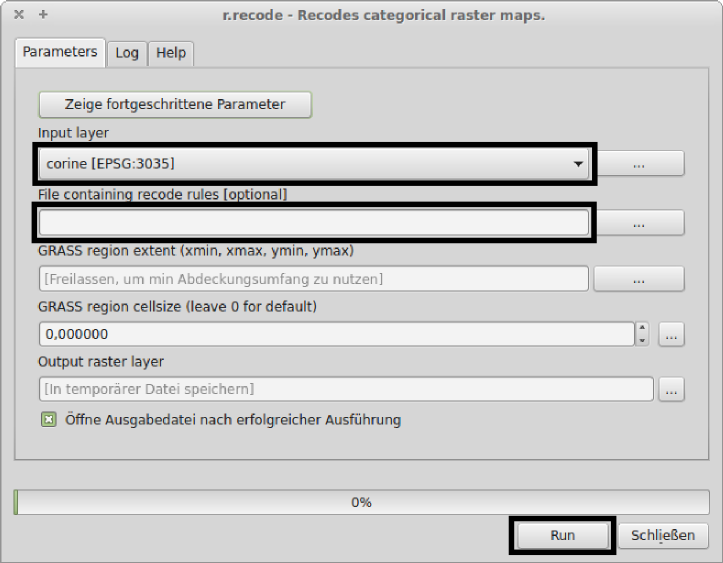
\includegraphics{qgis_recode.png}}
\caption{Der GRASS Algorithmus \emph{r.recode} in QGIS}\label{uebung3:figrecode}\end{figure}

Zunächst sollte man sicherstellen, dass unter \emph{Input layer} auch tatsächlich der Layer eingestellt ist, den man bearbeiten will. Als nächstes benötigt man eine Datei, welche die Regeln zur Reklassifikation beinhält. Diese kann mit einem einfachen Text Editor erstellt werden und muss dann in dem Feld \emph{File containing recode rules} eingetragen werden.

Die Aufschlüsselung, welche Klassen des Corine Datensatzes zu welcher größeren Klasse gehören, findet sich in der Datei \emph{clc\_legend.csv}.
Um nun beispielsweise eine Regel in die Reklassifikations-Regel-Datei einzutragen, welche alle ``Agricultural surfaces'' auf den Wert 1 zusammenfasst, müssen Sie zunächst in der \emph{clc\_legend.csv} nachsehen, welcher \emph{GRID\_CODE{}`s alle zu dieser Klasse gehören (siehe Abbildung :num:{}`\#figrecode\_csv}).
\begin{figure}[htbp]
\centering
\capstart

\scalebox{1.000000}{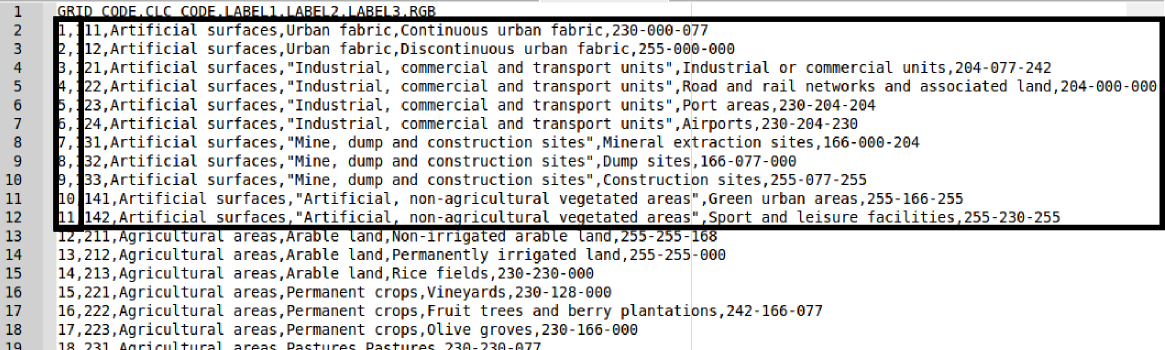
\includegraphics{recode_csv.png}}
\caption{Alle \emph{Agricultural surfaces} aus der Datei \emph{clc\_legend.csv} (gelber Rahmen) und deren GRID\_CODEs (roter Rahmen)}\label{uebung3:figrecode-csv}\end{figure}

Nun wissen wir, dass alle ursprünglichen Werte von 1 bis inklusive 11 zur Klasse \emph{Agricultural surfaces} gehören. Die Regel, die wir in unsere Regeldatei eintragen müssen lautet nun \code{1:11:1}. Dies ist so zu verstehen, dass alle Werte von \emph{1} bis \emph{11} in der neuen Datei den Wert \emph{1} zugewiesen bekommen. Man kann anstatt einer Zahl als neuen Wert auch den Wert \emph{NULL} eintragen. Dieser Wert beschreibt dann explizit, dass an dieser Stelle gar keine Messdaten vorliegen (selbst der Wert 0 könnte ja aus einer Messung stammen).

Die übrigen Einstellungen des r.recode Fensters kann man so belassen, wie sie sind. Mit einem Klick auf \emph{OK} wird der Vorgang gestartet und GRASS GIS berechnet die Reklassifikation. Nach Abschluss der Berechnung wird das Ergebnis automatisch in QGIS angezeigt.
\setbox0\vbox{
\begin{minipage}{0.95\linewidth}
\textbf{Aufgabe 8}

\medskip

\begin{itemize}
\item {} 
Verwenden Sie den Algorithmus \emph{r.recode} für eine Reklassifikation des Corine Rasters mit den folgenden Klassenzuweisungen nach oben beschriebenem Muster:
\begin{itemize}
\item {} 
Agrtificial surfaces -\textgreater{} 1

\item {} 
Agricultural areas -\textgreater{} 2

\item {} 
Forest and semi natural areas -\textgreater{} 3

\item {} 
Wetlands -\textgreater{} 4

\item {} 
Water bodies -\textgreater{} 5

\end{itemize}

\item {} 
Verändern Sie weiters die Darstellung des neu klassifizierten Layers den unten stehenden Angaben entsprechend.

\end{itemize}
\end{minipage}}
\begin{center}\setlength{\fboxsep}{5pt}\shadowbox{\box0}\end{center}

Das berechnete Ergebnis wird in QGIS zwar dargestellt, aber die Anzeige benötigt weitere Feineinstellungen um tatsächlich aussagekräftig zu sein.
Öffnen Sie das Eigenschafts Fenster des neu klassifizierten Layers (siehe Abbildung ) und welchseln Sie auf dessen \emph{Style (Stil)} Ansicht, sofern nicht bereits ausgewählt.
\begin{figure}[htbp]
\centering
\capstart

\scalebox{0.800000}{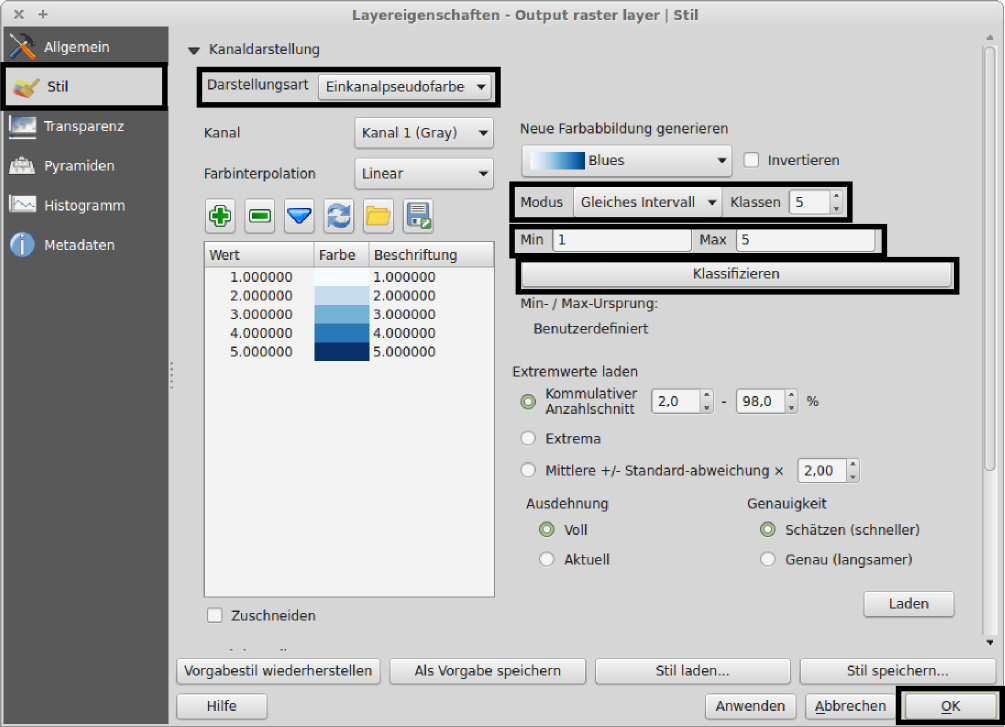
\includegraphics{qgis_recode_reclass.png}}
\caption{Die Darstellung des neu klassifizierten Layers muss mithilfe dessen Eigenschaftsfenster angepasst werden.}\label{uebung3:figrecode-reclass}\end{figure}

Wählen Sie abermals als gewünschte \emph{Darstellungsart} \emph{Singleband pseudocolor (Einkanalpseudofarbe)} aus. Unter \emph{Mode (Modus)} wählen Sie \emph{Equal Interval (Gleiches Intervall)} und geben bei \emph{Classes (Klassen)} den Wert \emph{5} vor, da wir bei Reklassifizieren auf genau 5 Klassen reduziert haben. Auch beim Feld \emph{Max} geben Sie \emph{5} ein, das Feld \emph{Min} bleibt bei \emph{1}.
Mit einem Klick auf den Knopf \emph{Classify (Klassifizieren)} werden nun 5 Anzeigeklassen mit der gewählten Farbpalette erstellt. Wenn Sie es bevorzugen, können Sie eine beliebige Farbpalette auswählen.
Wenn Sie das Fenster mit einem Klick auf \emph{OK} ganz schließen, können Sie die Veränderung der Anzeige in der QGIS Kartenanzeige sehen.


\section{Map-Algebra}
\label{uebung3:map-algebra}
Map-Algebra bezeichnet das mathematische Operieren mit Geodaten. Im einfachsten Fall versteht man darunter das Anwenden arithmetischer Operatoren (+, -, etc ...) auf die Werte von Rasterzellen.


\subsection{Lokale Operatoren}
\label{uebung3:lokale-operatoren}
Die folgende Berechnung nennt man eine Lokale Operation, weil sie pro Rasterzelle genau einmal ausgeführt wird und für das Ergebnis auch immer nur eine Rasterzelle herangezogen wird.
Es gibt in QGIS mehrere Möglichkeiten, Map-Algebra durchzuführen. Der fest in QGIS eingebaute Rasterrechner \footnote{
\href{https://docs.qgis.org/2.6/en/docs/user\_manual/working\_with\_raster/raster\_calculator.html}{https://docs.qgis.org/2.6/en/docs/user\_manual/working\_with\_raster/raster\_calculator.html}
} findet sich im Menü unter \emph{Raster} -\textgreater{} \emph{Raster Calculator (Rasterrechner)}.
\begin{figure}[htbp]
\centering
\capstart

\scalebox{1.000000}{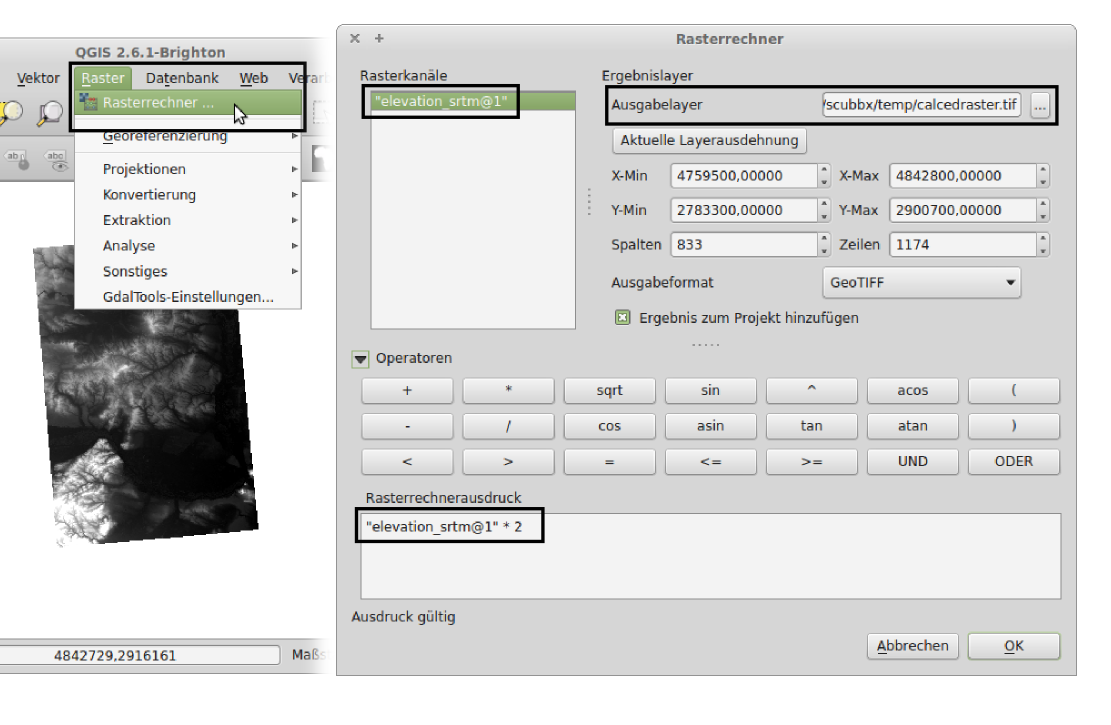
\includegraphics{qgis_rastercalc.png}}
\caption{Der Rasterkalkulator von QGIS mit dem Befehl zur Verdoppelung aller Rasterwerte des gewählten Rasters \emph{elevation\_srtm}}\label{uebung3:figqgisrastercalc}\end{figure}

Um beispielsweise alle Werte eines Rasters, der die Höhe in Metern gespeichert hat in Fuß umzurechnen, muss dieser Raster ausgewählt und mit 3,28 multipliziert werden. Die Syntax dazu ist in Abbildung \hyperref[uebung3:figqgisrastercalc]{ \ref*{uebung3:figqgisrastercalc}} dargestellt.


\subsection{Fokale Operatoren}
\label{uebung3:fokale-operatoren}
Fokale Operatoren (auch \emph{Neighborhood} Operatoren genannt) beziehen auch der aktuellen Rasterzelle umliegende Zellen mit ein. Der QGIS eigene Rasterrechner bietet nur Optionen für Lokale Operationen an. Daher greifen wir wieder auf externe Algorithmen aus der \emph{Processing} Toolbox zurück.

Der GRASS Algorithmus namens \emph{r.mapcalculator} bietet die Möglichkeit, solche Fokalen Operationen durchzuführen (siehe Abbildung \hyperref[uebung3:figqgisgrassrastercalc]{ \ref*{uebung3:figqgisgrassrastercalc}}).
\begin{figure}[htbp]
\centering
\capstart

\scalebox{0.600000}{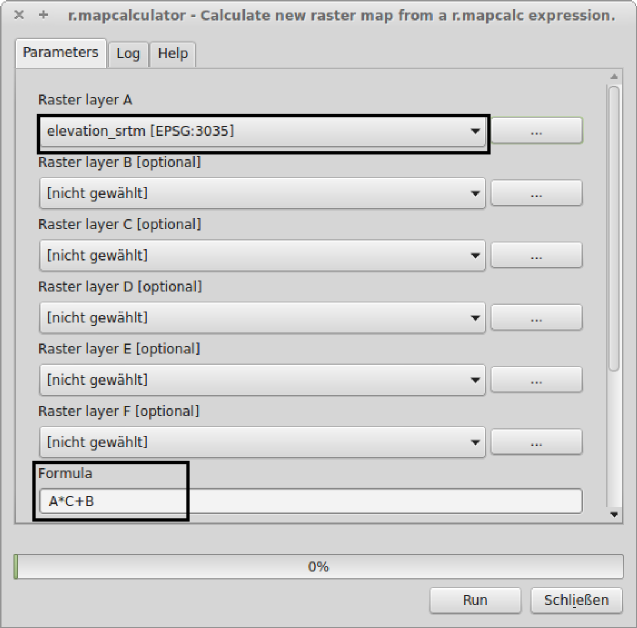
\includegraphics{qgis_grass_rastercalc.png}}
\caption{Der GRASS Algorithmus \emph{r.mapcalculator} von GRASS Gis}\label{uebung3:figqgisgrassrastercalc}\end{figure}

Im Feld \emph{Raster layer A} wählt man den Rasterlayer aus, welcher in der Formel mit der Variable \emph{A} angesprochen wird. In diesem Fall ist dies das SRTM Höhenmodell.
Weiter unten kann im Feld \emph{Formula} die Formel eingetragen werden. Auch hier könnte man, um von Meter auf Fuß umzurechnen, einfach \code{A * 3,28} eingetragen werden.
Um nun eine Fokale Operation durchzuführen, sagen wir, immer die zwei nebeneinander liegenden Rasterzellen zusammenzuaddieren, muss man folgendes eintragen: \code{A + A{[}-1,0{]}}.
Die Syntax dieser Fromel ist so zu verstehen, dass \emph{A} immer die konrete, aktuell berechnete Rasterzelle unseres Raterlayers darstellt. Wenn nun \emph{A{[}-1,0{]}} angegeben wird bewirkt dies, dass die Rasterzelle \emph{links} unserer aktuellen Zelle verwendet wird. Der Wert \emph{-1} verschiebt unser Berechnungsfenster also um eine Zelle nach links. Der zweite Wert \emph{0}, beschreibt die Verschiebung nach Oben oder Unten. In unserem Fall bedeutet 0, dass wir auf der selben Höhe bleiben, also keine Verschiebung vornehmen.
Die gesamte Formel bewirkt also, dass immer der Wert der gerade aktuellen Zelle mit dem Wert der Zelle links davon zusammengezählt wird. Eine genauere Beschreibung aller Möglichkeiten, die der Algorithmus \emph{r.mapcalculator} bietet kann in dessen Online-Hilfe \footnote{
\href{http://grass.osgeo.org/grass64/manuals/r.mapcalc.html}{http://grass.osgeo.org/grass64/manuals/r.mapcalc.html}
} nachgeschlagen werden.

Mit einem Klick auf \emph{OK} wird die Prozedur gestartet. Das hier genannte Beispiel macht nur wenig Sinn, auch das Ergebnis wird nur sichtbar, wenn man weit hineinzoomt. Allerdings wird dadurch verständlich, wie man unter Einsatz längerer Formeln kompliziertere Berechnungen durchführen kann.
\setbox0\vbox{
\begin{minipage}{0.95\linewidth}
\textbf{Aufgabe 9}

\medskip


Glätten Sie den SRTM-Raster mit Hilfe des Map Calculators, indem Sie Mittelwerte einer 3x3-Nachbarschaft bilden. (Hinweis: für genau solch eine Aufgabe existiert bereits ein eigener Algorithmus namens \emph{r.neighbors}, der einem das Tippen der Formel abnimmt)

Um ein aussagekräftiges Bild für die Abgabe zu erhalten müssen Sie unter Umständen nahe in den geglätteten Datensatz hineinzoomen um einen Unterschied zum Original feststellen zu können.
\end{minipage}}
\begin{center}\setlength{\fboxsep}{5pt}\shadowbox{\box0}\end{center}


\subsection{Masken}
\label{uebung3:masken}
Eine Maske dient dazu, nur bestimmte Bereiche eines Rasters in die Berechnung einzuschließen. Im standard QGIS Rasterrechner, im Menü \emph{Raster} -\textgreater{} \emph{Raster Calculator (Rasterrechner)}, kann eine Maske beispielsweise mit folgendem Ausdruck definiert werden: \code{("elevation\_srtm@1" \textgreater{} 300) * "elevation\_srtm@1"}
Mit dieser Formel werden nur Bereich beibehalten, die einen Wert über 300 besitzen. Der Teil \emph{(``elevation\_srtm@1'' \textgreater{} 300)} gibt entweder eine \emph{1} als Ergebnis, wenn der jeweilige Rasterzellenwert über 300 liegt, oder eine 0, wenn dieser darunter liegt. Wenn wir dieses Ergebnis nun mit dem Originalraster multiplizieren (\emph{* ``elevation\_srtm@1''}) bewirkt das, dass alles, was unter 300 Metern liegt, folglich den Wert 0 zugewiesen bekommt. Alle anderen Werte bleiben so, wie sie sind.
\setbox0\vbox{
\begin{minipage}{0.95\linewidth}
\textbf{Aufgabe 10}

\medskip


Erzeugen Sie mit oben beschriebener Methode eine Karte, welche nur Gebiete über 200 Metern anzeigt.
\end{minipage}}
\begin{center}\setlength{\fboxsep}{5pt}\shadowbox{\box0}\end{center}

Sie können mithilfe einer Vorlage auch Bereiche aus einem Raster herausschneiden. Um nur das Gebiet von Wien aus den SRTM Höhendaten zu erhalten, stellen Sie zunächst sicher, dass Sie das zuvor besprochenen Bezirksgrenzen Shapefile geladen haben. Mit dem \emph{Processing} Algorithmus \emph{Clip raster by mask layer} (in das Such-Feld der \emph{Processing (Verarbeitungswerkzeuge)} Toolbox eingeben) können wir nun diesen Bereich aus unserer Rasterkarte ausschneiden.
\setbox0\vbox{
\begin{minipage}{0.95\linewidth}
\textbf{Aufgabe 11}

\medskip


Schneiden Sie den Bereich von Wien aus dem SRTM Höhenlayer und aus dem zuvor reklassifizierten Corine Datensatz aus.
\end{minipage}}
\begin{center}\setlength{\fboxsep}{5pt}\shadowbox{\box0}\end{center}


\subsection{Zonale Operatoren}
\label{uebung3:zonale-operatoren}
Zonale Größen werden über fest vordefinierte Zonen aggregiert. Diese Zonen können beliebige Gebiete von beliebiger Ausdehnung sein. Es gibt verschiedene zonale Algorithmen in der \emph{Processing} Toolbox wie \emph{r.average}, \emph{r.median} oder \emph{r.mode}. Ein etwas allgemeinerer Befehl für Zonale Operationen ist \emph{r.statistics}, dieser hat zur Zeit allerdings einen Bug, welcher ihn unbrauchbar macht. Wir werden uns daher auf die spezielleren Befehle beschränken.

Bei den GRASS Algorithmen, welche über die Processing Toolbox verfügbar sind, beschreibt das Feld \emph{Base raster layer} jenen Layer, der die Zonen, für die ein Wert berechnet werden soll, vorgibt. Unter \emph{Cover raster layer} wird der Layer ausgewählt, aus dem die jeweilige Statistik berechnet wird (siehe Abbildung \hyperref[uebung3:figqgisraverage]{ \ref*{uebung3:figqgisraverage}}).
\begin{figure}[htbp]
\centering
\capstart

\scalebox{0.600000}{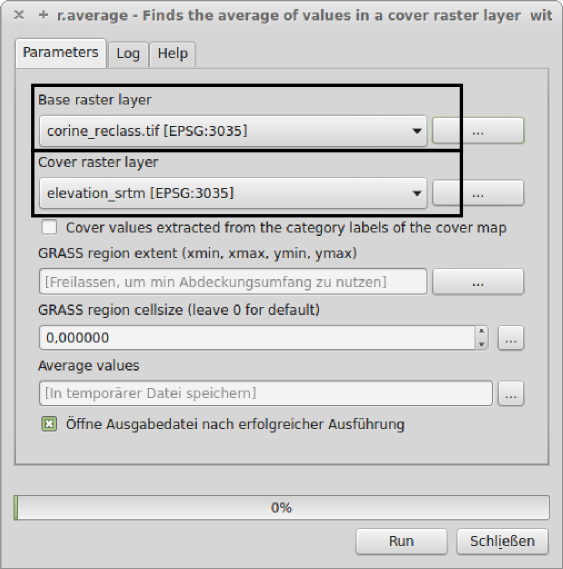
\includegraphics{qgis_raverage.png}}
\caption{Der GRASS Algorithmus \emph{r.average} zur Berechnung von zonalen Durchschnittswerten}\label{uebung3:figqgisraverage}\end{figure}
\setbox0\vbox{
\begin{minipage}{0.95\linewidth}
\textbf{Aufgabe 12}

\medskip


Ermitteln Sie die durchschnittliche Höhe für jede der fünf reklassifizierten Corine Klassen innerhalb des Wiener Gemeindegebietes. Hierfür eignet sich der Algorithmus ``r.average''. Der zuvor erstellte reklassifizierte Corine Raster dient dabei als Vorgabe für die Zonen, die Höhen können aus den SRTM Daten berechnet werden.
\end{minipage}}
\begin{center}\setlength{\fboxsep}{5pt}\shadowbox{\box0}\end{center}


\subsection{Kombination mehrerer Raster}
\label{uebung3:kombination-mehrerer-raster}
Mit dem QGIS Rasterrechner können auch mehrere Layer auf einmal bearbeitet und kombiniert werden (auf ähnliche Weise ist dies auch mit dem \emph{r.mapcalc} Rasterrechner möglich). Im Fenster der Rasterrechnes sind in der Liste mit der Beschriftung \emph{Rasterkanäle} alle verfügbaren Rasterdaten aufgelistet. Diese Einträge können Sie in Ihrer Formal beliebig kombinieren.
\setbox0\vbox{
\begin{minipage}{0.95\linewidth}
\textbf{Aufgabe 13}

\medskip


Finden Sie alle \emph{künstlichen} Flächen, die \emph{höher als 200 Meter} liegen. Verwenden Sie als Grundlage den reklassifizierten Corine Raster und den SRTM Raster. Erinnern Sie sich, wir haben die Klasse \emph{1} verwendet, um künstliche Flächen im Corine Datensatz zu klassifizieren (``Artificial surfaces'').
\end{minipage}}
\begin{center}\setlength{\fboxsep}{5pt}\shadowbox{\box0}\end{center}


\section{Sichtbarkeitsanalysen}
\label{uebung3:sichtbarkeitsanalysen}
Sichtbarkeitsanalysen werden in Kombination mit Höhenmodellen und 3D Stadtmodellen für die Planung neuer Gebäude und Infrastruktur eingesetzt. Der \emph{Processing} Toolbox Befehl \emph{r.los}, dargestellt in Abbildung \hyperref[uebung3:figqgisrlos]{ \ref*{uebung3:figqgisrlos}}, berechnet Sichtbarkeitszonen in Abhängigkeit von einem gegebenen Punkt und eines Höhenrasters.
\begin{figure}[htbp]
\centering
\capstart

\scalebox{0.700000}{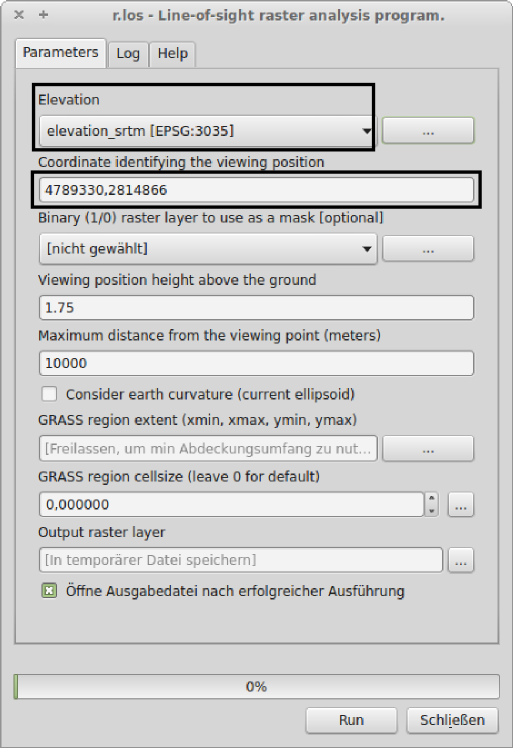
\includegraphics{qgis_rlos.png}}
\caption{Der GRASS Algorithmus \emph{r.los} zur Berechnung der Sichtbarkeit von einem Punkt (``Line of Sight'')}\label{uebung3:figqgisrlos}\end{figure}
\setbox0\vbox{
\begin{minipage}{0.95\linewidth}
\textbf{Aufgabe 14}

\medskip


Berechnen Sie die Sichtbarkeitszonen um den Punkt mit den Koordinaten \emph{4789330,2814866} unter Zuhilfenahme des SRTM Rasters für die Höhen.
\end{minipage}}
\begin{center}\setlength{\fboxsep}{5pt}\shadowbox{\box0}\end{center}


\section{Abgabe}
\label{uebung3:abgabe}
Beantworten Sie die Fragen im Text und führen Sie die genannten Aufgaben aus. Vergessen Sie nicht, zu jeder Aufgabe ein Bild des Endergebnisses abzuspeichern. Fügen Sie alle erstellten Bilder in eine pdf Datei und kommentieren Sie die Ergebnisse kurz. Die Abgabe erfolgt im TUWEL.


\chapter{Übung 4: Vektordaten}
\label{uebung4:ubung-4-vektordaten}\label{uebung4::doc}

\section{GIS Vektordaten}
\label{uebung4:gis-vektordaten}
Neben sogenannten topologischen Dateiformaten ist der heutzutage gebräuchlichste Weg um vektorbasierte GIS Daten abzuspeichern das \emph{OGC Simple Features Modell} \footnote{
\href{http://grass.osgeo.org/grass64/manuals/r.mapcalc.html}{http://grass.osgeo.org/grass64/manuals/r.mapcalc.html}
} .
Dieses erlaubt die Beschreibung von Geoinformation mit den drei typen: \emph{Punkte}, \emph{Linien} und \emph{Polygone} (siehe Abbildung \hyperref[uebung4:figvector]{ \ref*{uebung4:figvector}}). Des weiteren ist es noch möglich, Gruppen aus jeweils diesen Elementen zu definieren, welche sich dann entsprechend \emph{Multi-Punkte}, \emph{Multi-Linien} und \emph{Multi-Polygone} nennen.
\begin{figure}[htbp]
\centering
\capstart

\scalebox{0.700000}{
\includegraphics{vector.png}}
\caption{Die drei primären Datentypen laut dem OGC Simple Feature Standard}\label{uebung4:figvector}\end{figure}

Es lässt sich nahezu jedes 2-dimensionale Objekt mit diesen drei Typen beschreiben.
Jedes einzelne Element (ein Punkt, eine Linie, ein Polygon) kann zusätzlich mit einem oder mehreren Attributen versehen werden. Üblicherweise ist das eine Laufnummer (\emph{ID} genannt) und oftmals eine Typenbezeichnung. Die genaue Auswahl dieser Eigenschaften ist vom Anwendungsfall abhängig und vollständig dem Benutzer überlassen.
Diese Attribute lassen sich einfach in einer Tabelle darstellen. Jede Reihe dieser Tabelle beschreibt einen Eintrag im Datensatz. Solch ein einzelner Eintrag wird im Allgemeinen als \emph{Feature} bezeichnet, egal ob es sich um einen Punkt, eine Linie oder ein Polygon handelt.

Es gibt Ansätze, den 3-dimensionalen Raum zu beschreiben, wir werden uns in der Übung aber auf den klassischen Fall einfacher Kartendarstellungen in 2D beschränken.


\section{Das Shapefile}
\label{uebung4:das-shapefile}
Als Standard zur Speicherung von Vektordaten hat sich in der GIS Welt das \emph{Shapefile} Format durchgesetzt. Dieses Format wurde ursprünglich von der Firma ESRI \footnote{
\href{http://www.esri.com}{http://www.esri.com}
} entwickelt. Da der Standard für die Benutzung dieses Dateiformats kostenlos freigegeben wurde, hat sich dieses Format weltweit durchgesetzt und ist, obwohl es inzwischen heillos veraltet ist, immer noch der de-facto Standard. Es gibt bereits eine Unzahl an weiteren Vektorformaten, die das Shapefile ablösen wollen, doch konnte sich bis jetzt keines davon durchsetzen.

Eine bezeichnende Eigenschaft eines Shapefiles ist, dass sich ein einzelnes Shapefile aus mehreren Dateien zusammensetzt. Sehen Sie sich den Link unter \footnote{
\href{http://de.wikipedia.org/wiki/Shapefile}{http://de.wikipedia.org/wiki/Shapefile}
} an, um die Bedeutung der einzelnen Dateien zu verstehen.
\setbox0\vbox{
\begin{minipage}{0.95\linewidth}
\textbf{Aufgabe 15}

\medskip


Benennen Sie die Datei, welche für die Speicherung der Geometriedaten zuständig ist.
\end{minipage}}
\begin{center}\setlength{\fboxsep}{5pt}\shadowbox{\box0}\end{center}

Wir hatten in der vorhergehenden Übung bereits kurz Kontakt zu einem Vektordatensatz: die Bezirksgrenzen von Wien.


\section{Laden und Selektieren von Vektorobjekten}
\label{uebung4:laden-und-selektieren-von-vektorobjekten}
Wir sehen uns nun den Datensatz \emph{SCHULEOGD} aus den Übungsdaten an. Dieser Datensatz ist in einem andern Koordinatensystem als das von uns gewünschte gespeichert. Somit ist es zunächst nötig, diesen Datensatz, so wie in der vorhergehenden Übung beschrieben, in das von uns gewählte ETRS89 Koordinatensystem umzuspeichern und diese umprojezierten Daten zu laden.
\setbox0\vbox{
\begin{minipage}{0.95\linewidth}
\textbf{Aufgabe 16:}

\medskip

\begin{itemize}
\item {} 
Laden Sie den aus der vorhergehenden Übung umprojezierten \emph{BEZIRKSGRENZEOGD} Datensatz oder projezieren Sie diesen erneut um.

\item {} 
Projezieren Sie den Datensatz \emph{SCHULEOGD} in das ETRS89 Koordinatensystem um und laden Sie diesen, sofern dies nicht automatisch geschehen ist.

\item {} 
Stellen Sie sicher, dass als das projektweite Kooridnatensystem ebenfalls ETRS89 eingestellt ist.

\end{itemize}
\end{minipage}}
\begin{center}\setlength{\fboxsep}{5pt}\shadowbox{\box0}\end{center}

Stellen Sie sicher, dass der \emph{SCHULEOGD} Layer über dem mit den Gemeindebezirken liegt. Um die Layer unter oder über einen andern zu schieben, kann man ihn mit der Maus an die Position ziehen, an der er dargestellt werden soll.

Sobald die beiden Vektorlayer geladen sind, sind sie in der \emph{Layers (Layer)} Liste links vom QGIS Kartenfenster zu sehen. Auswahl- und Abfrageoperationen werden immer auf dem Layer ausgeführt, welcher gerade ausgewählt ist.
\begin{figure}[htbp]
\centering
\capstart

\scalebox{1.000000}{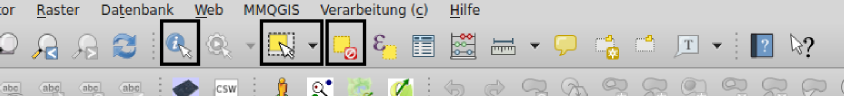
\includegraphics{vectorselect.png}}
\caption{Die Icons zum (1) Abfragen von Attributen, zum (2) Auswählen von einzelnen Features und zum (3) Aufheben der Auswahl}\label{uebung4:figvectorselect}\end{figure}

Abbildung \hyperref[uebung4:figvectorselect]{ \ref*{uebung4:figvectorselect}} zeigt die Kommandos in der Symbolleiste, um Attribute eines Features abzufragen, ein Feature auszuwählen und um die Auswahl wieder aufzuheben.
Um beispielsweise den 2. Bezirk auszuwählen, muss das entsprechende Icon in der Symbolleiste ausgewählt werden und der 2. Bezirk im Kartenfenster angeklickt werden. Dieser färbt sich Gelb, was anzeigt, dass er ausgewählt wurde.

Wie zuvor erwähnt, sind die Attribute eines Shapefiles (wie auch bei fast allen anderen vektor-basierten GIS Dateiformaten) in einer Tabelle gespeichert, welche mit den Kartendaten verknüpft ist. In QGIS kann man sich diese Tabelle ansehen, indem man mit der Rechten Maustaste auf den entsprechenden Layer klickt und im daraufhin erscheinenden Menü den Eintrag \emph{Open Attribute Table} auswählt (siehe Abbildung \hyperref[uebung4:figattrib]{ \ref*{uebung4:figattrib}}).
\begin{figure}[htbp]
\centering
\capstart

\scalebox{1.000000}{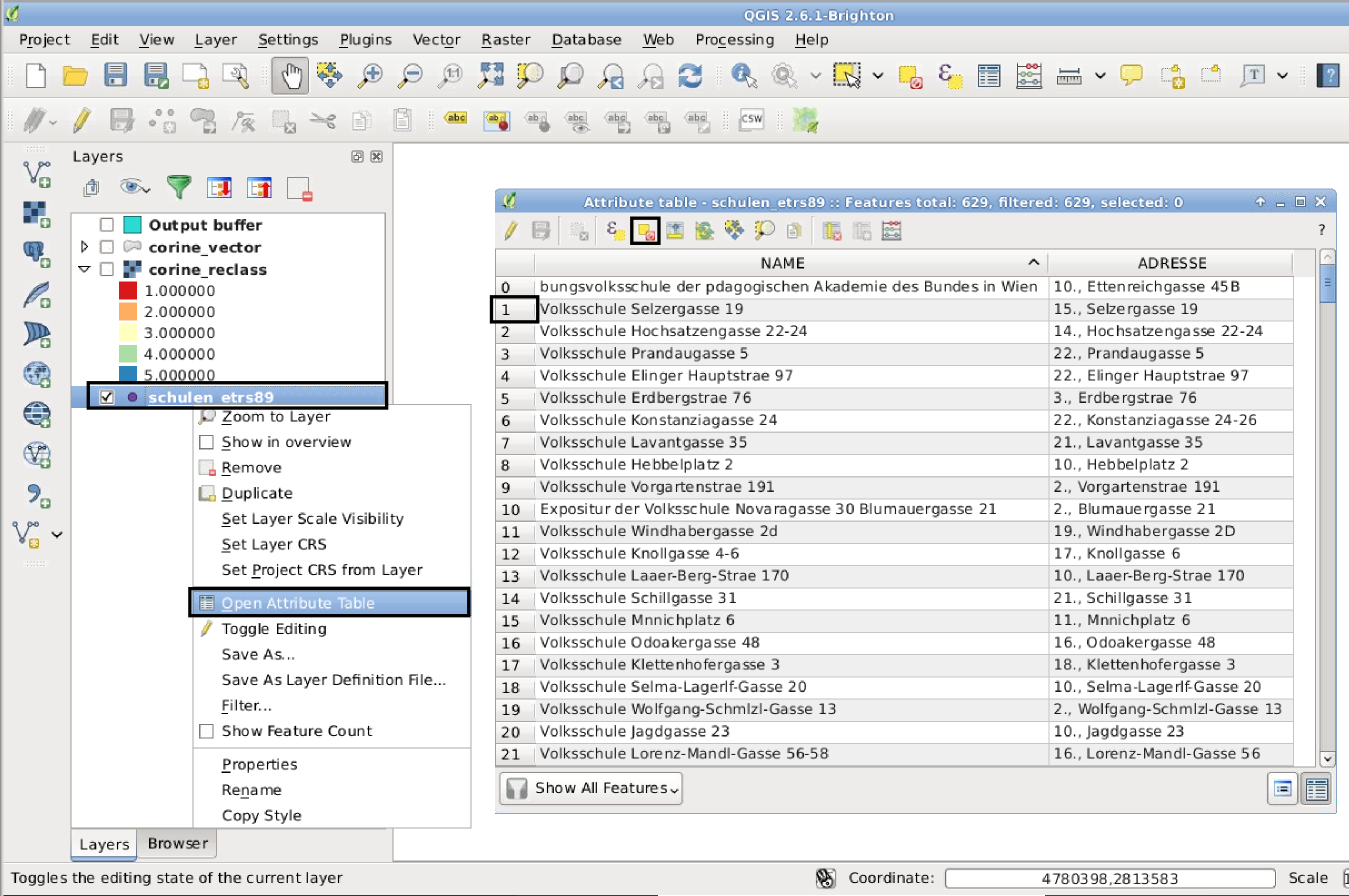
\includegraphics{qgis_attrib.png}}
\caption{Die Attributtabelle eines Vektorlayers}\label{uebung4:figattrib}\end{figure}

Im Fall der Wiener Schulen kann man erkennen, dass jede Schule (Zeilen in der Tabelle) jeweils ein Attribut mit den Namen \emph{NAME} und \emph{ADRESSE} bestitzt. Wenn man auf eine eine Zahl ganz links in der Tabelle klickt, wird genau dieses Feature ausgewählt. Das ist nützlich, wenn man ein bestimmtes Feature mit genau einer bestimmten Adresse bearbeiten will. Mit einem Klick auf den \emph{Unselect all} Knopf, wird diese Auswahl wieder aufgehoben.

Es ist möglich, Features eines Layers anhand deren Lage im Bezug zu einem anderen Feature auszuwählen. Der Befehl dazu findet sich im Menü unter \emph{Vector} -\textgreater{} \emph{Research Tools (Forschungswerkzeuge)} -\textgreater{} \emph{Select by Location (Nach Position auswählen)}.
\begin{figure}[htbp]
\centering
\capstart

\scalebox{1.000000}{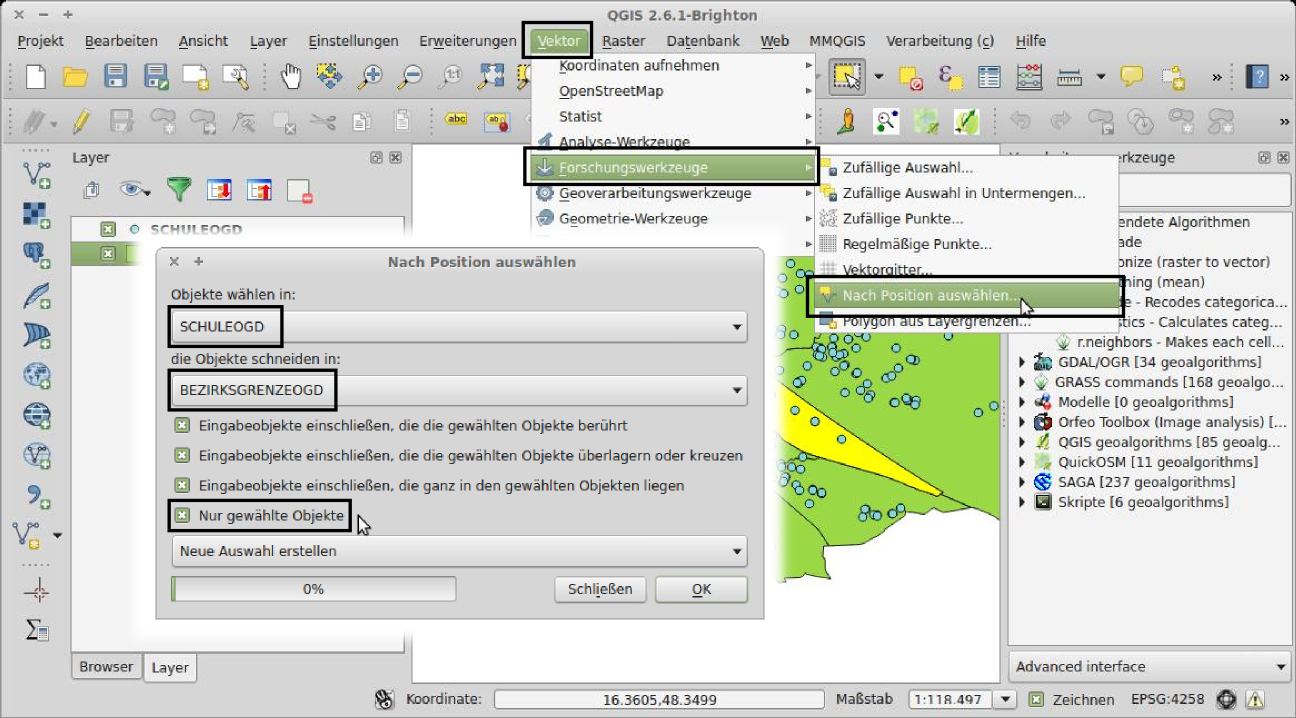
\includegraphics{qgis_selectloc.png}}
\caption{Die Funktion zur Auswahl von Objekten nach ihrer Lage}\label{uebung4:figqgisvectorselect}\end{figure}

Es öffnet sich das Fenster wie in Abbildung \hyperref[uebung4:figqgisvectorselect]{ \ref*{uebung4:figqgisvectorselect}} dargestellt.
Im Feld \emph{Select features in (Objekt wählen in)} wird der Layer eingestellt, aus welchem Objekte ausgewählt werden. Das Feld \emph{that intersect features in (die Objekte schneiden in)} beschreibt den Layer, der die Grenzen beinhält, aus innerhalb derer ausgewählt wird. Eine wichtige Option, welche in unserem Fall ausgewählt sein muss, ist \emph{Only selected features (Nur gewählte Objekte)}.

Um nur eine Auswahl an Features in eine neue Datei abzuspeichern, nutzen wir abermals die \emph{Save as... (Speichern als ...)} Funktion, die mithilfe eines Rechtsklicks auf den jeweiligen Layer gefunden werden kann.
\begin{figure}[htbp]
\centering
\capstart

\scalebox{1.000000}{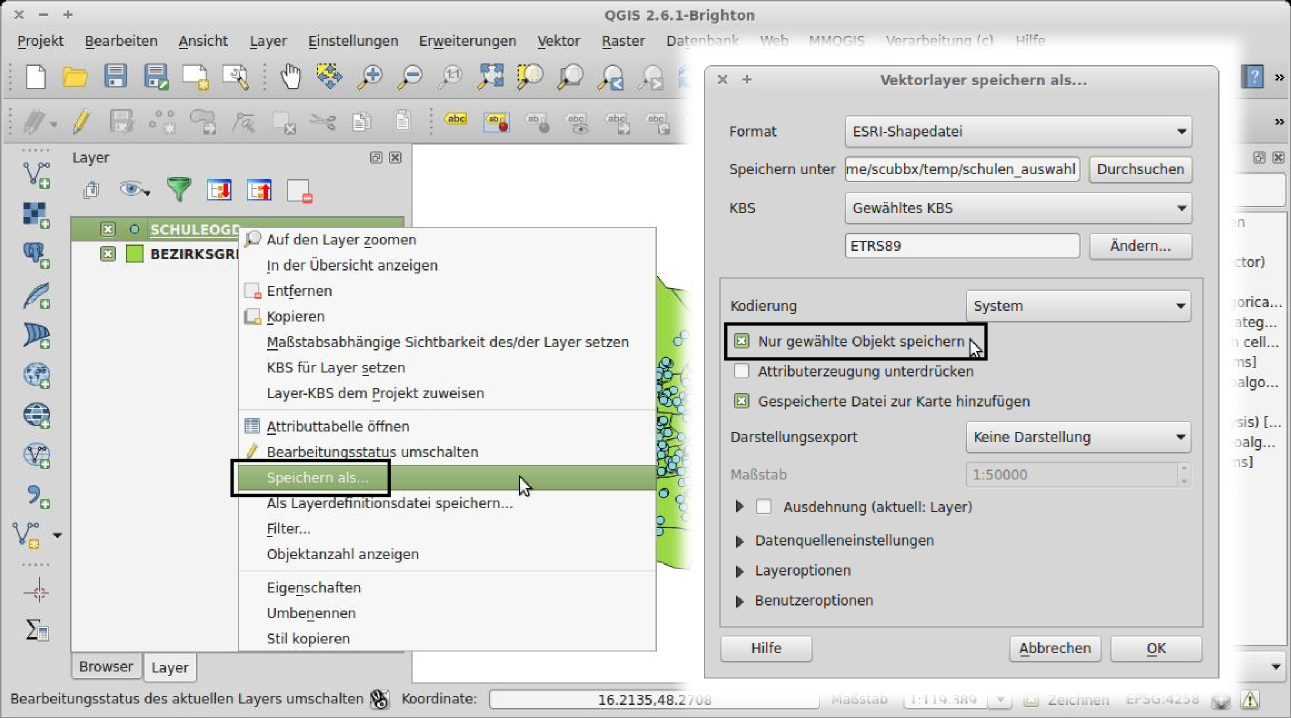
\includegraphics{qgis_saveselection.png}}
\caption{Um nur die ausgewählten Features zu speicher, genügt die Auswahl einer Option im \emph{Save as... (Speichern als ...)} Dialog}\label{uebung4:figqgissaveselect}\end{figure}

Abbildung \hyperref[uebung4:figqgissaveselect]{ \ref*{uebung4:figqgissaveselect}} zeigt das Fenster, in welchem die Option \emph{Save only selected features} ausgewählt sein muss, damit nur die derzeit ausgewählten Features gespeichert werden.
\setbox0\vbox{
\begin{minipage}{0.95\linewidth}
\textbf{Aufgabe 17}

\medskip

\begin{itemize}
\item {} 
Wählen Sie mit der oben beschriebenen Methode alle Schlulen aus, welche im 2. Wiener Gemeindebezirk liegen.

\item {} 
Speichern Sie nur diese Schulen in einer eigenen Datei ab und laden Sie diese, sofern dies nicht bereits automatisch geschehen ist.

\end{itemize}
\end{minipage}}
\begin{center}\setlength{\fboxsep}{5pt}\shadowbox{\box0}\end{center}


\section{Buffer Operationen}
\label{uebung4:buffer-operationen}
Für viele Aufgaben sind sogenannte Bufferzonen hilfreich - zum Beispiel können Bufferzonen entlang von Straßenachsen gebildet werden, um die Beeinträchtigung durch den Lärm in der Nähe der Straße abzuschätzen. Buffer können um beliebige Vektorobjekte gebildet werden. Für manche Aufgaben sind auch richtungsabhängige Buffer sinnvoll - zum Beispiel könnte der Lärm entlang einer bestimmten Richtung durch Bäume oder Mauern gedämpft werden und somit die Bufferzone entlang dieser Richtung kleiner sein.
\begin{figure}[htbp]
\centering
\capstart

\scalebox{0.700000}{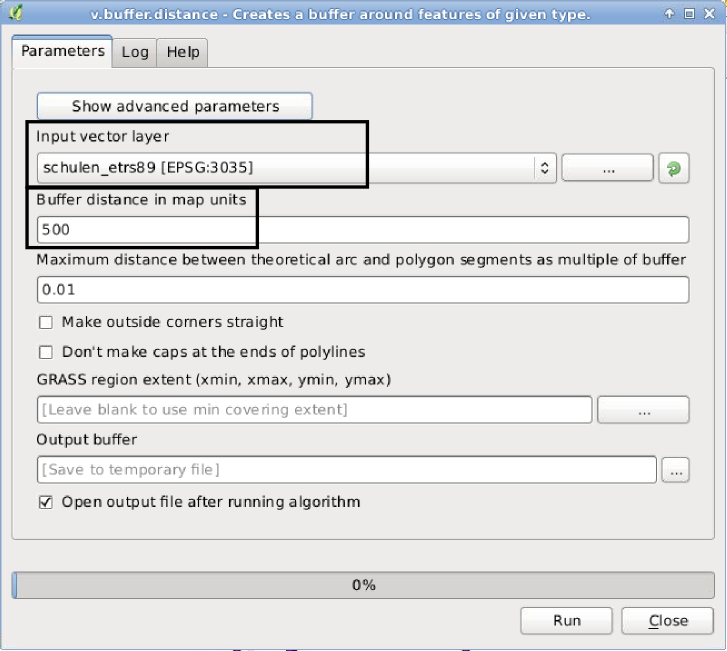
\includegraphics{qgis_vgbuffer.png}}
\caption{Die \emph{Processing} Funktion \emph{v.buffer.distance}}\label{uebung4:figbuffer}\end{figure}

Abbildung \hyperref[uebung4:figbuffer]{ \ref*{uebung4:figbuffer}} zeigt die \emph{Processing} Funktion \emph{v.buffer.distance}. Unter \emph{Buffer distance in map units} kann die Distanz für die Bufferzone angegeben werden. Wichtig dabei zu beachten ist, dass man unbedingt einen entsprechend in Metern projezierten Layer verwendet, da ansonsten die Pufferdistanz in Grad verstanden wird. In diesem Fall erzeugt man schnell Pufferzonen, die um die halbe Weltkugel reichen.
Das Ergebnis dieser Operation ist ein oder mehrere Polygon in einem Layer, welche die Bufferzonen um den Eingabelayer darstellen.
\setbox0\vbox{
\begin{minipage}{0.95\linewidth}
\textbf{Aufgabe 18}

\medskip


Gesucht ist die Zone, die innerhalb von 500 Metern zu einer Schule liegt. Nutzen sie einen Buffer, um diese Zonen zu berechnen und darzustellen.
\end{minipage}}
\begin{center}\setlength{\fboxsep}{5pt}\shadowbox{\box0}\end{center}


\section{Raster in Vektoren Umwandeln}
\label{uebung4:raster-in-vektoren-umwandeln}
In vielen Situationen ist es sinnvoll, einen Rasterlayer in einen Vektorlayer umzuwandeln. Dabei wird ein Raster in seiner Qualität nicht verbessert. In den meisten Fällen werden aus einem Raster Polygone erzeugt, es existieren jedoch auch Funktionen, Linien oder Punkte aus einem Raster zu erzeugen.

Um solch eine Umwandlung durchzuführen, gibt es abermals mehrere Möglichkeiten. Wir werden jene benutzen, welche fest in QGIS verankert ist und im Menü unter \emph{Raster} -\textgreater{} \emph{Conversion (Konvertierung)} -\textgreater{} \emph{Polygonize (Vektorisieren)} aufgerufen werden kann. Wir werden nun beispielsweise den zuvor von uns neu klassifizierten CORINE Landbedeckungslayer vekotrisieren. Dazu muss dieser zunächst geöffnet werden, sofern er nicht schon geladen ist. Das Fenster der Vektorisierungsfunktion sieht wie in Abbildung \hyperref[uebung4:figvectorize]{ \ref*{uebung4:figvectorize}} dargestellt aus.
\begin{figure}[htbp]
\centering
\capstart

\scalebox{0.700000}{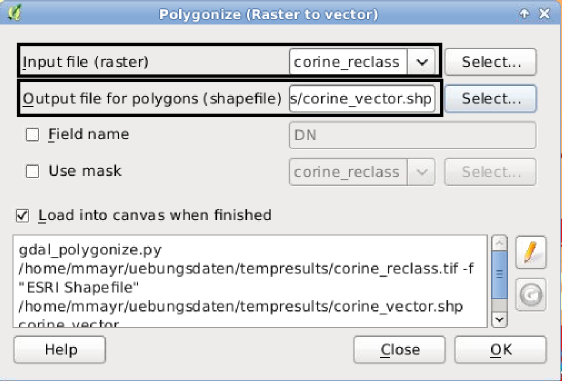
\includegraphics{qgis_vectorize.png}}
\caption{Mit der Funktion \emph{Polygonize (Vektorisieren)} kann man Raster in Vektor-Polygone umwandeln}\label{uebung4:figvectorize}\end{figure}

Es muss ein Dateiname zum Abspeichern angegeben werden. Mit einem Klick auf \emph{OK} wird der Prozess gestartet und die vektorisierte Variante wird geladen. Wenn wir einen Blick auf die Attributtabelle des neu erstellen Vektorlayers werfen, sehen wir, dass genau ein Attribut mit dem Namen \emph{DN} existiert. Dies ist der Wert, welchen wir pro Klasse beim Reklassifizieren des CORINE Layers eingegeben hatten (siehe Abbildung \hyperref[uebung4:figselectattr]{ \ref*{uebung4:figselectattr}}).
\begin{figure}[htbp]
\centering
\capstart

\scalebox{0.700000}{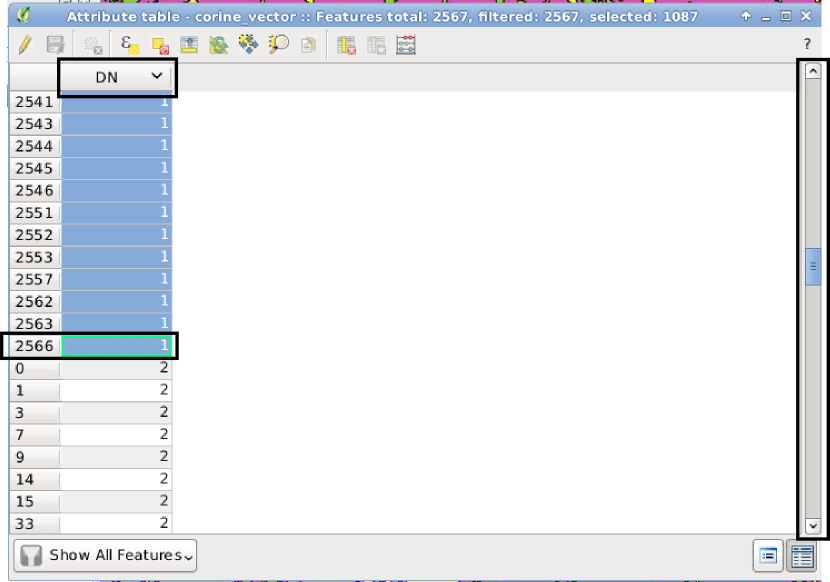
\includegraphics{qgis_selectattr.png}}
\caption{Wenn man die Tabelle nach der gewünschten Spalte sortiert, kann man leicht alle gewünschten Elemente einer Klasse auswählen}\label{uebung4:figselectattr}\end{figure}

Um nun alle Features einer bestimmten Klasse auszuwählen, sollten wir zunächst die Tabelle nach der Spalte \emph{DN} sortieren. Dazu klicken wir einfach darauf. Nun kann mit einem Klick auf die (in unserem Fall) Zahl \emph{4} der erste Eintrag ausgewählt werden. Nun scrollen wir so weit nach unten, bis wir den letzten Eintrag mit dem Wert \emph{1} sehen (in unserem Fall trägt dieser die Nummer \emph{2566}). Um nun alle Einträge zwischen diesem und dem zuvor von uns Markierten auszuwählen, klicken wir auf den letzten Eintrag, während wir die \emph{Umschalt} Taste gedrückt halten.
Wenn die Attributtabelle geschlossen wird, bleibt die Auswahl weiterhin bestehen. Man kann dies daran erkennen, dass alle von uns ausgewählten Flächen Gelb eingefärbt sind. Nun kann man, ähnlich wie mit den Schulen des 2. Bezirks zuvor, diese Auswahl in einer eigenen Datei abspeichern.
\setbox0\vbox{
\begin{minipage}{0.95\linewidth}
\textbf{Aufgabe 19}

\medskip


Gesucht ist der Standort für eine neue Schule. Die Schule soll
\begin{itemize}
\item {} 
mindestens 500 Meter von allen anderen Schulen entfernt sein und

\item {} 
in einem Gebiet mit der CORINE Klassifikation ``künstliche Flächen''

\end{itemize}

liegen. Dazu können Sie den zuvor berechneten Bufferlayer der Schulen und die vektorisierte CORINE Klassifikation, die nur die Klasse 1 enthält, benutzen. Erinnern Sie sich, die Klasse 1 beschreibt genau alle ``künstlichen Flächen''.

Erzeugen Sie diese beiden Datensätze und setzen Sie gleich mit der folgenden Aufgabe fort. Sie müssen für diese Aufgabe kein Bild oder Screenshot anfertigen.
\end{minipage}}
\begin{center}\setlength{\fboxsep}{5pt}\shadowbox{\box0}\end{center}


\section{Overlay Operationen}
\label{uebung4:overlay-operationen}
Mithilfe von Overlay Operationen können meherere Layer miteinander kombiniert werden. Dazu gibt es verschiedene Varianten, oft als \emph{or}, \emph{not} oder \emph{xor} bezeichnet. Diese verschneiden zwei Vektorlayer mit unterschiedlichen Resultaten. Wir werden uns die \emph{or} Operation näher ansehen, in QGIS wird diese auch als \emph{Clip} bezeichnet.
Die \emph{Clip} Funktion findet man im Menü unter \emph{Vector} -\textgreater{} \emph{Geoprocessing (Geoverarbeitungswerkzeuge)} -\textgreater{} \emph{Clip (Clipper)} und sieht wie auf Abbildung \hyperref[uebung4:figclip]{ \ref*{uebung4:figclip}} dargestellt aus.
\begin{figure}[htbp]
\centering
\capstart

\scalebox{0.700000}{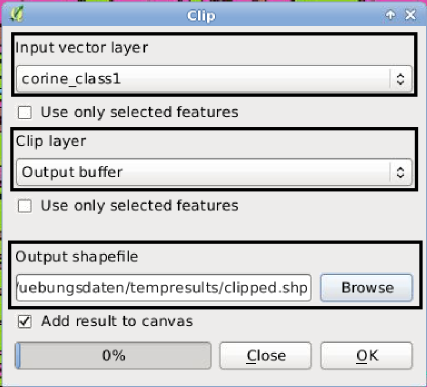
\includegraphics{qgis_clip.png}}
\caption{Mit der \emph{Clip (Clipper)} Funktion können gemeinsame Flächen zwei verschiedener Layer berechnet werden}\label{uebung4:figclip}\end{figure}
\setbox0\vbox{
\begin{minipage}{0.95\linewidth}
\textbf{Aufgabe 20}

\medskip


Um einen gemeinsamen Datensatz, der zuvor genannte Kriterien (Aufgabe 19) für eine neue Schule erfüllt, zu erzeugen, kombinieren Sie den Pufferdatensatz mit dem vektorisierten der CORINE Klasse 1.

\textbf{Hinweis:} Da wir nicht die gemeinsame Fläche der 500 Meter Zone um bestehende Schulen (nicht gesucht) und der künstlichen Flächen (gesucht) suchen, ist die \emph{clip} Funktion hier die falsche Wahl. Ein richtiges Ergebnis erzielen wir mit der \emph{Difference (Differenz)} Funktion, welche uns die Bereiche berechnet, die sich nicht überlappen.
\end{minipage}}
\begin{center}\setlength{\fboxsep}{5pt}\shadowbox{\box0}\end{center}


\section{Delaunay-Triangulation und Voronoi-Diagramme}
\label{uebung4:delaunay-triangulation-und-voronoi-diagramme}
Eine Delaunay-Triangulation verbindet gegebene Punkte zu Dreiecken, sodass der Umkreis eines jeden Dreiecks keinen weiteren Punkt enthält. Delaunay-Triangulationen werden für die Erstellung von digitalen Geländemodellen (DGM) verwendet, indem man die Punkte, an denen die Geländehöhen beobachtet wurden, trianguliert und die Höhen zwischen den Punkten interpoliert.

Bildet man zu jeder Kante der Triangulation Ihre duale Kante, also die Streckensymmetralen der Dreieckskante, so erhält man das zugehörige Voronoi-Diagramm. Das Voronoi-Diagramm unterteilt ein Gebiet in sogenannte Voronoi-Zellen. Voronoi-Diagramme verden in GIS Anwendungen für die Modellierung von Einzugsgebieten verwendet.

Mit den Algorithmen \emph{v.delaunay} und \emph{v.voronoi} aus der \emph{Processing Toolbox} lassen sich Delaunay-Triangulation und Voronoi-Diagramme berechnen.
\setbox0\vbox{
\begin{minipage}{0.95\linewidth}
\textbf{Aufgabe 21}

\medskip


Gesucht ist die nächste Schule zu Ihrem Wohnort. Berechnen Sie dazu zunächst die Voronoi-Diagramme der Schulen innerhab Wiens. Dann markieren Sie mit der am Beginn besprochenen Auswahlfunktion jene Zelle des Voronoi-Diagramms, in welcher Ihre Wohnadresse liegt.
\end{minipage}}
\begin{center}\setlength{\fboxsep}{5pt}\shadowbox{\box0}\end{center}


\section{Abgabe}
\label{uebung4:abgabe}
Beantworten Sie die Fragen, fügen Sie alle Ergebnisse in eine pdf Datei und kommentieren Sie kurz die Ergebnisse. Vergessen Sie nicht, bei jeder Aufgabe ein Bild anzufertigen, das Ihr Ergebnis zeigt. Die Abgabe erfolgt im TUWEL.


\chapter{Übung 5: Netzwerkoperationen}
\label{uebung5:ubung-5-netzwerkoperationen}\label{uebung5::doc}
In dieser Übung wird ein Auszug aus OpenStreetMap (OSM) verwendet. Unter \footnote{
\href{http://www.geofabrik.de}{http://www.geofabrik.de}
} werden täglich aktuelle Auszüge aus dem OSM-Datensatz im Shapefile-Format bereitgestellt. Die Daten für diese Übung wurden aufgrund der Größe auf das Wiener Gemeindegebiet eingeschränkt.


\section{Datenaufbereitung}
\label{uebung5:datenaufbereitung}
Laden Sie zunächst den Datensatz \emph{vie\_roads} aus den Übungsdaten in QGIS. Wie sie sehen können, beinhält dieser alle Straßen und Bahngleise innerhalb Wiens.
Uns interessieren aber nur die Begehbaren Straßen. Daher müssen wir auch nur diese herausfiltern.

QGIS bietet dafür bei Vektorlayern eine interessante Funktion namens \emph{Filter}. Mit einem Rechtsklick auf den gewünschten Layer kann diese ausgewählt werden (siehe Abbildung \hyperref[uebung5:figfilter]{ \ref*{uebung5:figfilter}}).
\begin{figure}[htbp]
\centering
\capstart

\scalebox{1.000000}{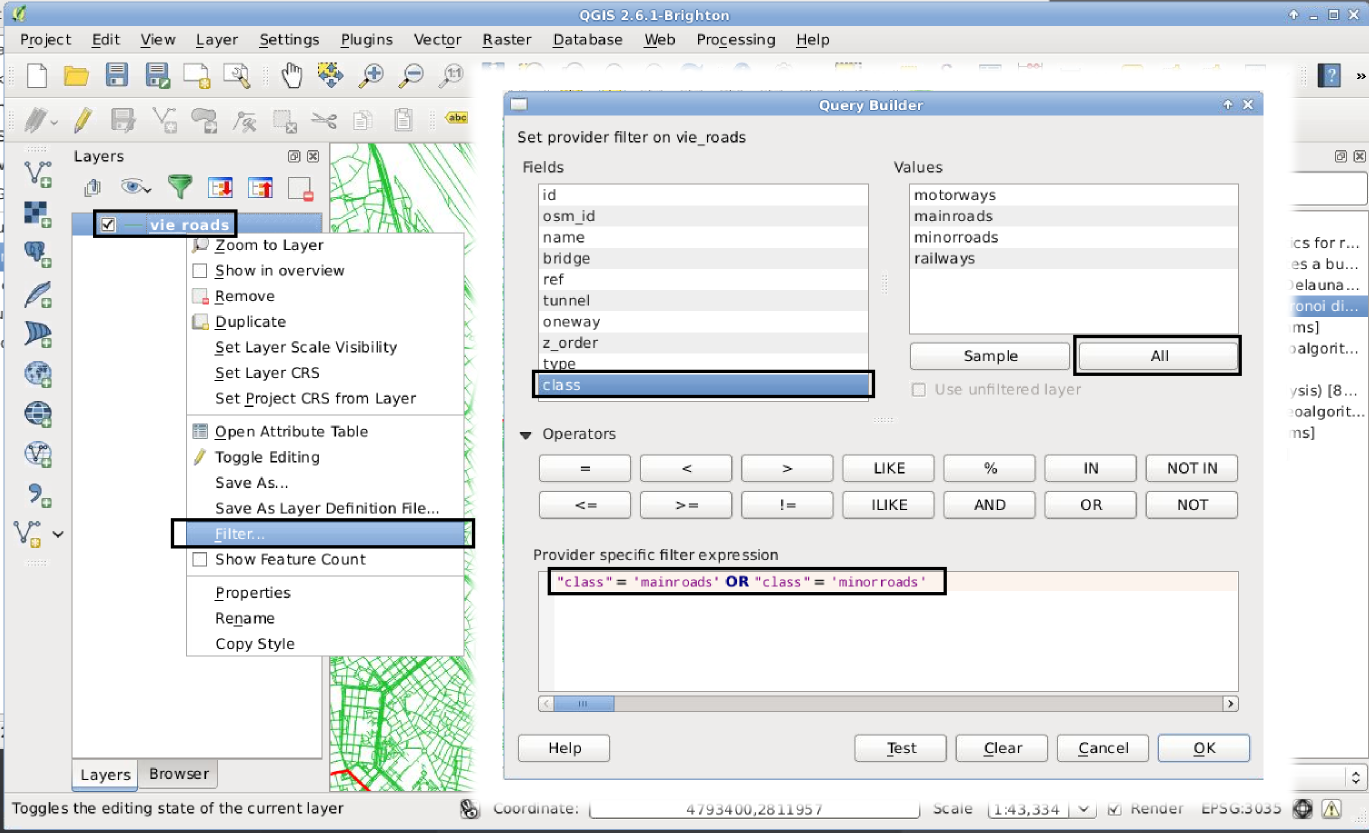
\includegraphics{qgis_filter.png}}
\caption{Die \emph{Filter} Funktion in QGIS}\label{uebung5:figfilter}\end{figure}

Nun kann mit einer Syntax ähnlich jener von SQL ein Filter angegeben werden, nach dem die Daten gefiltert werden. Für QGIS sieht es danach so aus, als ob die Datei tatsächlich nur jene Features beinhalten würde, die die Filter Funktion passieren.
Die Liste mit dem Titel \emph{Fields (Felder)} listet alle verfügbaren Attributklassen auf. Uns interessiert derzeit das Feld \emph{class}, also sollten wir es auswählen. Mit einem Klick auf den Knopf \emph{All (Alle)} werden im darüberliegenden Feld alle Attributwerte der ausgewählten Attributklasse aufgelistet. In unserem Fall geschieht dies sehr schnell, wenn man aber mit Datensätzen mit Millionen von Einträgen arbeitet, sollte man besser den Knopf mit der Aufschrift \emph{Sample (Stichprobe)} benutzen. Anderenfalls kann die Prozedur zum Laden aller möglichen Einträge sehr viel Zeit in Anspruch nehmen.

Wir können nun erkennen, dass in der Attributklasse \emph{class} nur vier verschiedene Einträge vorkommen: \emph{motorways}, \emph{mainroads}, \emph{minorroads} und \emph{railways}. In unserem Fall interessieren uns nur die \emph{mainroads} und \emph{minorroads}, denn nur diese können auch zu Fuß begangen werden.
Um diese herauszufiltern, schreiben wir folgende Formel in das Feld mit dem Titel \emph{Provider specific filter expression (Datenlieferanten spezifischer Ausdruck)}:

Nach einem Klick auf \emph{OK}, wird die Anzeige aktualisiert und nur mehr Haupt- und Nebenstraßen gezeigt.
\setbox0\vbox{
\begin{minipage}{0.95\linewidth}
\textbf{Aufgabe 22}

\medskip


Filtern Sie alle Autobahnen und Bahnschienen aus dem Datensatz.
\end{minipage}}
\begin{center}\setlength{\fboxsep}{5pt}\shadowbox{\box0}\end{center}


\section{Kürzester Weg}
\label{uebung5:kurzester-weg}
Der kürzeste Weg wird mit dem Dijkstra-Algorithmus \footnote{
\href{http://de.wikipedia.org/wiki/Dijkstra-Algorithmus}{http://de.wikipedia.org/wiki/Dijkstra-Algorithmus}
} berechnet. Im QGIS Plugin \emph{Road graph plugin} (Straßengraph-Erweiterung) ist dieser Algorithmus enthalten. Die Funktion wird mit Hilfe eines andockbaren Fensters bereitgestellt, das im Menü unter \emph{View} (Ansicht) -\textgreater{} \emph{Panels} (Bedienfelder) -\textgreater{} \emph{Shortest Path} (Kürzester Weg) aktiviert werden kann, sofern es nicht schon sichtbar ist. Falls sich diese Option nich im Menü finden lässt, muss sie zuerst im Pluginmanager aktiviert werden.
\begin{figure}[htbp]
\centering
\capstart

\scalebox{1.000000}{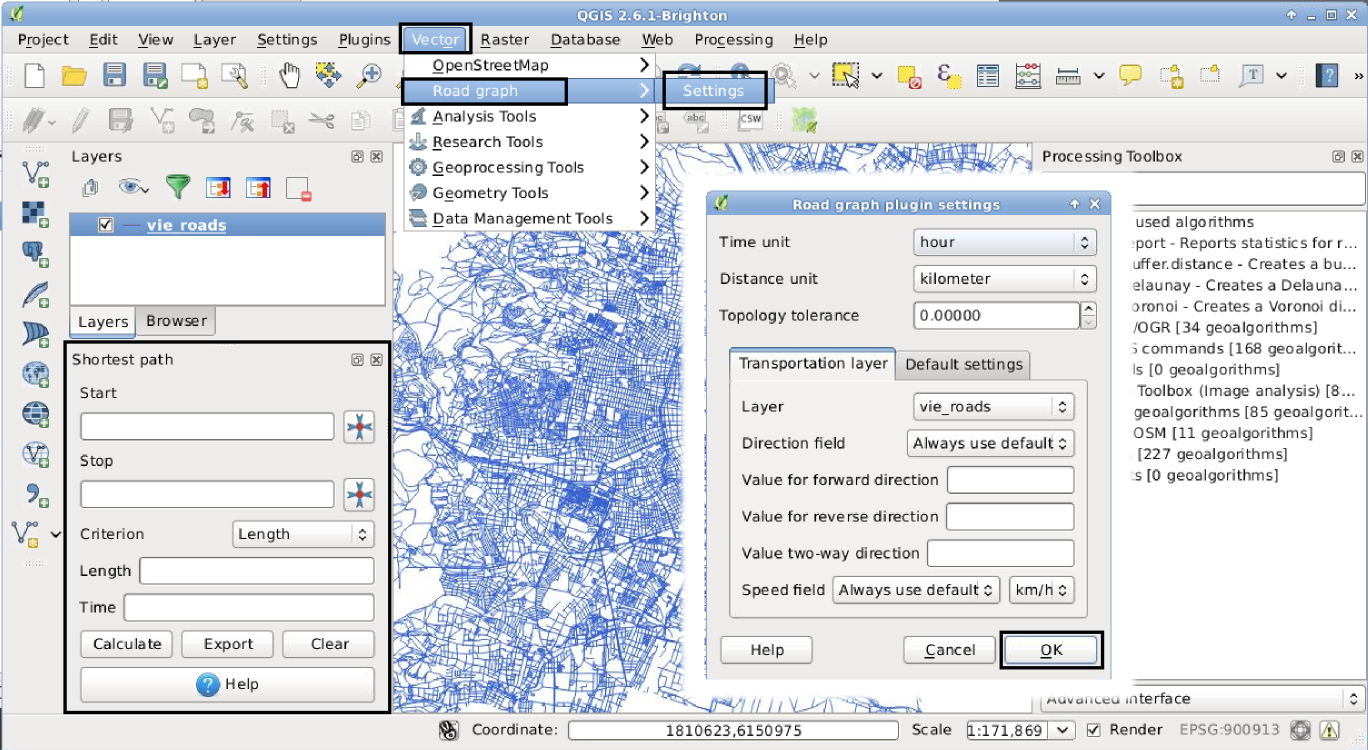
\includegraphics{qgis_route.png}}
\caption{Die \emph{Shortest-Path} Funktion in QGIS}\label{uebung5:figroute}\end{figure}

Wie in Abbildung \hyperref[uebung5:figroute]{ \ref*{uebung5:figroute}} dargestellt, müssen zunächst die Einstellungen des Plugins geöffnet werden, damit bestimmte Standardoptionen automatisch gesetzt werden. Hier kann man diverse Optionen angeben, welche wir so lassen, wie sie sind. Das Fenster kann mit einem Klick auf \emph{OK} geschlossen werden.

Um nun die kürzeste Route zwischen zwei Punkten zu berechnen, klicken wir zunächst auf das erste Fadenkreuz neben dem Feld, welches mit \emph{Start} beschriftet ist, und dann auf die Stelle in der Karte, an der wir starten wollen. Wir führen den Gleichen Schritt mit dem Fadenkreuz unterhalb des ersten aus, um den Endpunkt zu markieren. Um die Berechnung zu starten, klicken Sie auf \textbf{Calculate (Berechnen)}.
\setbox0\vbox{
\begin{minipage}{0.95\linewidth}
\textbf{Aufgabe 23}

\medskip


Berechnen Sie die kürzeste Route zwischen Ihrem Wohnort und der TU Wien (oder dem Karlsplatz).
\end{minipage}}
\begin{center}\setlength{\fboxsep}{5pt}\shadowbox{\box0}\end{center}


\section{Abgabe}
\label{uebung5:abgabe}
Fügen Sie alle ausgegebenen Dateien in eine pdf Datei und kommentieren Sie kurz die Ergebnisse. Beantworten Sie die Fragen im Text. Die Abgabe erfolgt über TUWEL.



\renewcommand{\indexname}{Stichwortverzeichnis}
\printindex
\end{document}
